% Created 2023-02-26 Sun 00:00
% Intended LaTeX compiler: pdflatex
\documentclass[twoside]{article}
        \usepackage[accepted]{aistats2023}
\usepackage[citestyle=authoryear-comp, maxcitenames=2, maxbibnames=99, doi=false, isbn=false, eprint=false, backend=bibtex, hyperref=true, url=false, natbib=true, style=authoryear-comp]{biblatex}
\addbibresource{zotero-library.bib}
\usepackage{bm}
\usepackage{amsmath,amssymb,amsfonts}
\usepackage[makeroom]{cancel}
\usepackage[disable]{todonotes}
\usepackage{subcaption}
\usepackage{caption}
\captionsetup[figure]{font=footnotesize}
\usepackage{mathtools}
\usepackage{algpseudocode}
\usepackage{algorithm}
\usepackage{tikz,pgfplots}
\usetikzlibrary{bayesnet}
\usepackage[utf8]{inputenc}
\DeclareUnicodeCharacter{2212}{−}
\usepgfplotslibrary{groupplots,dateplot}
\usetikzlibrary{patterns,shapes.arrows}
\pgfplotsset{compat=newest}
\usepackage{fontawesome5}
\usepackage[colorlinks=true,linkcolor=blue,allcolors=blue]{hyperref}
\usepackage[capitalise,nameinlink]{cleveref}
\newcommand{\defeq}{\vcentcolon=}
\newtheorem{definition}{Definition}[section]
\newtheorem{assumption}{Assumption}[section]
\newtheorem{theorem}{Theorem}[section]
\newtheorem{lemma}{Lemma}[section]
\crefname{section}{Sec.}{Secs.}
\crefname{algorithm}{Alg.}{Algs.}
\crefname{appendix}{App.}{Apps.}
\crefname{definition}{Def.}{Defs.}
\crefname{table}{Tab.}{Tabs}
\DeclareMathOperator{\R}{\mathbb{R}}
\DeclareMathOperator{\E}{\mathbb{E}}
\DeclareMathOperator{\V}{\mathbb{V}}
\DeclareMathOperator{\K}{\mathbf{K}}
\newcommand{\numData}{\ensuremath{t}}
\newcommand{\numEpisodes}{\ensuremath{e}}
\newcommand{\numTimesteps}{\ensuremath{t}}
\newcommand{\numInd}{\ensuremath{m}}
\newcommand{\stateDim}{\ensuremath{d}}
\newcommand{\controlDim}{\ensuremath{f}}
\newcommand{\modeInd}{\ensuremath{k}}
\newcommand{\modeDesInd}{\ensuremath{\text{des}}}
\newcommand{\testInd}{\ensuremath{*}}
\newcommand{\NumData}{\ensuremath{\MakeUppercase{\numData}}}
\newcommand{\NumInd}{\ensuremath{\MakeUppercase{\numInd}}}
\newcommand{\StateDim}{\ensuremath{{D_x}}}
\newcommand{\ControlDim}{\ensuremath{{D_u}}}
\newcommand{\ModeInd}{\ensuremath{\MakeUppercase{\modeInd}}}
\newcommand{\NumEpisodes}{\MakeUppercase{\numEpisodes}}
\newcommand{\NumTimesteps}{\MakeUppercase{\numTimesteps}}
\newcommand{\singleData}[1]{\ensuremath{#1_{\numData}}}
\newcommand{\allData}[1]{\ensuremath{\MakeUppercase{#1}}}
\newcommand{\singleOutputK}{\ensuremath{\mode{\singleOutput}}}
\newcommand{\singleDataDim}[1]{\ensuremath{_{\stateDim}#1_{\numData}}}
\newcommand{\singleDim}[1]{\ensuremath{#1_{\stateDim}}}
\newcommand{\mode}[1]{\ensuremath{#1_{\modeInd}}}
\newcommand{\modeDes}[1]{\ensuremath{#1^{\modeDesInd}}}
\newcommand{\singleDimiMode}[2]{\ensuremath{\tensor*[_#2^\modeInd]{#1}{}}}
\newcommand{\singleDimMode}[1]{\ensuremath{\singleDimiMode{#1}{\stateDim}}}
\newcommand{\singleDimModeData}[1]{\ensuremath{\tensor*[_\stateDim^\modeInd]{#1}{_\numData}}}
\newcommand{\state}{\ensuremath{\mathbf{x}}}
\newcommand{\control}{\ensuremath{\mathbf{u}}}
\newcommand{\x}{\ensuremath{\mathbf{x}}}
\newcommand{\y}{\ensuremath{y}}
\newcommand{\dataset}{\ensuremath{\mathcal{D}}}
\newcommand{\singleInput}{\ensuremath{\x_{\numData-1}}}
\newcommand{\singleOutput}{\ensuremath{\singleData{\y}}}
\newcommand{\allInput}{\ensuremath{\allData{\x}}}
\newcommand{\allOutput}{\ensuremath{\MakeUppercase{\y}}}
\newcommand{\singleState}{\ensuremath{\state_{\numData-1}}}
\newcommand{\singleControl}{\ensuremath{\control_{\numData-1}}}
\newcommand{\allState}{\ensuremath{\allData{\state}}}
\newcommand{\allControl}{\ensuremath{\allData{\control}}}
\newcommand{\noiseVar}{\ensuremath{\sigma}}
\newcommand{\noiseVarK}{\ensuremath{\mode{\noiseVar}}}
\newcommand{\noiseVarOneK}{\ensuremath{\singleDimiMode{\noiseVar}{1}}}
\newcommand{\noiseVarDK}{\ensuremath{\singleDimiMode{\noiseVar}{\StateDim}}}
\newcommand{\noiseVardK}{\ensuremath{\singleDimMode{\noiseVar}}}
\newcommand{\modeVar}{\ensuremath{\alpha}}
\newcommand{\modeVarn}{\ensuremath{\singleData{\modeVar}}}
\newcommand{\ModeVar}{\ensuremath{\bm{\modeVar}}}
\newcommand{\modeVarK}{\ensuremath{\modeVarn=\modeInd}}
\newcommand{\ModeVarK}{\ensuremath{\ModeVar_{\modeInd}}}
\newcommand{\gatingFunc}{\ensuremath{h}}
\newcommand{\GatingFunc}{\ensuremath{\mathbf{\gatingFunc}}}
\newcommand{\latentFunc}{\ensuremath{f}}
\newcommand{\LatentFunc}{\ensuremath{\mathbf{\latentFunc}}}
\newcommand{\F}{\ensuremath{\MakeUppercase{\mathbf{\latentFunc}}}}
\newcommand{\gatingParams}{\ensuremath{\bm\phi}}
\newcommand{\expertParams}{\ensuremath{\bm\theta}}
\newcommand{\gatingParamsK}{\ensuremath{\mode{\bm\phi}}}
\newcommand{\expertParamsK}{\ensuremath{\mode{\bm\theta}}}
\newcommand{\Z}{\ensuremath{\mathbf{Z}}}
\newcommand{\derivative}[1]{\ensuremath{\dot{#1}}}
\newcommand{\stateDerivative}{\ensuremath{\derivative{\state}}}
\newcommand{\pFk}{\ensuremath{p\left(\Fk \mid \allInput, \expertParams\right)}}
\newcommand{\pF}{\ensuremath{p\left(\F \mid \allInput, \expertParams\right)}}
\newcommand{\pfk}{\ensuremath{p\left(\fk \mid \allInput, \expertParamsK \right)}}
\newcommand{\pfknd}{\ensuremath{p\left(\fknd \mid \allInput\right)}}
\newcommand{\pFkGivenUk}{\ensuremath{p\left(\Fk \mid \uFk \right)}}
\newcommand{\pYkGivenFku}{\ensuremath{p\left(\allOutput \mid \ModeVarK, \uFk \right)}}
\newcommand{\qF}{\ensuremath{q\left(\F \right)}}
\newcommand{\qFu}{\ensuremath{q\left(\uF \right)}}
\newcommand{\qFku}{\ensuremath{q\left(\uFk \right)}}
\newcommand{\pFku}{\ensuremath{p\left(\uFk \mid \zFk \right)}}
\newcommand{\pFkuGivenX}{\ensuremath{p\left(\uFk \mid \zFk \right)}}
\newcommand{\pFuGivenX}{\ensuremath{p\left(\uF \mid \zF \right)}}
\newcommand{\qFk}{\ensuremath{q\left(\Fk \right)}}
\newcommand{\qfk}{\ensuremath{q\left(\fk \right)}}
\newcommand{\qfkn}{\ensuremath{q\left(\fkn \right)}}
\newcommand{\qfn}{\ensuremath{q\left(\fn \right)}}
\newcommand{\pFkGivenFku}{\ensuremath{p\left(\Fk \mid \uFk \right)}}
\newcommand{\pfkGivenFku}{\ensuremath{p\left(\fkn \mid \uFk \right)}}
\newcommand{\pykGivenFku}{\ensuremath{p\left(\singleOutput \mid \modeVarK, \uFk \right)}}
\newcommand{\pYGivenUX}{\ensuremath{p\left(\allOutput \mid \uF, \allInput \right)}}
\newcommand{\pYGivenU}{\ensuremath{p\left(\allOutput \mid \uF \right)}}
\newcommand{\pY}{\ensuremath{p\left(\allOutput \right)}}
\newcommand{\pykGivenx}{\ensuremath{p\left(\singleOutput \mid \modeVarK, \singleInput \right)}}
\newcommand{\pykGivenxNegF}{\ensuremath{p\left(\singleOutput \mid \modeVarK, \singleInput, \neg\Fk \right)}}
\newcommand{\pykGivenfk}{\ensuremath{p\left(\singleOutput \mid \modeVarK, \fkn \right)}}
\newcommand{\pykGivenfkd}{\ensuremath{p\left(\singleOutput \mid \modeVarK, \fknd \right)}}
\newcommand{\pYkGivenFk}{\ensuremath{p\left(\allOutput \mid \ModeVarK, \Fk \right)}}
\newcommand{\pYkGivenX}{\ensuremath{p\left(\allOutput \mid \ModeVarK, \allInput \right)}}
\newcommand{\pYGivenX}{\ensuremath{p\left(\allOutput \mid \allInput \right)}}
\newcommand{\PrA}{\ensuremath{\Pr\left(\ModeVarK \right)}}
\newcommand{\Pra}{\ensuremath{\Pr\left(\modeVarK \right)}}
\newcommand{\PaGivenhx}{\ensuremath{P\left(\modeVarn \mid \hn, \singleInput \right)}}
\newcommand{\PraGivenx}{\ensuremath{\Pr\left(\modeVarn \mid \singleInput \right)}}
\newcommand{\PraGivenhx}{\ensuremath{\Pr\left(\modeVarK \mid \hn, \singleInput \right)}}
\newcommand{\PraGivenxNegH}{\ensuremath{\Pr\left(\modeVarK \mid \singleInput, \neg\Hall \right)}}
\newcommand{\PrAGivenX}{\ensuremath{\Pr\left(\ModeVarK \mid \allInput \right)}}
\newcommand{\pHGivenX}{\ensuremath{p\left(\Hall \mid \allInput\right)}}
\newcommand{\pHkGivenX}{\ensuremath{p\left(\Hk \mid \allInput\right)}}
\newcommand{\Kkxx}{\mode{\mathbf{K}}_{d, \allInput\allInput}}
\newcommand{\ddK}{\ensuremath{\partial^2\K_{**}}}
\newcommand{\dK}{\ensuremath{\partial\K_{*}}}
\newcommand{\Kxx}{\ensuremath{\K_{}}}
\newcommand{\iKxx}{\ensuremath{\Kxx^{-1}}}
\newcommand{\dKz}{\ensuremath{\partial\K_{*\zH}}}
\newcommand{\Kzz}{\ensuremath{\K_{\zH\zH}}}
\newcommand{\iKzz}{\ensuremath{\Kzz^{-1}}}
\newcommand{\HDes}{\ensuremath{\MDes{\GatingFunc}}}
\newcommand{\uHDes}{\ensuremath{\MDes{\uH}}}
\newcommand{\pDes}{\ensuremath{p\left( \uHDes \mid \zHDes \right)}}
\newcommand{\qDes}{\ensuremath{q\left( \uHDes \right)}}
\newcommand{\mDes}{\ensuremath{\MDes{\mathbf{m}}}}
\newcommand{\SDes}{\ensuremath{\MDes{\mathbf{S}}}}
\newcommand{\singleTest}[1]{\ensuremath{#1_{\testInd}}}
\newcommand{\testInput}{\ensuremath{\singleTest{\state}}}
\newcommand{\Jac}{\ensuremath{\mathbf{J}}}
\newcommand{\testJac}{\ensuremath{\singleTest{\Jac}}}
\newcommand{\muJac}{\ensuremath{\mu_{\Jac}}}
\newcommand{\covJac}{\ensuremath{\Sigma_{\Jac}}}
\DeclareMathOperator*{\argmax}{argmax}
\newcommand{\diag}{\mathop{\mathrm{diag}}}

    \newcommand{\mboxparagraph}[1]{\paragraph{#1}\mbox{}\\}
    \newcommand{\mboxsubparagraph}[1]{\subparagraph{#1}\mbox{}\\}
\date{}
\title{}
\begin{document}

% If your paper is accepted and the title of your paper is very long,
% the style will print as headings an error message. Use the following
% command to supply a shorter title of your paper so that it can be
% used as headings.
%
\runningtitle{Mode-constrained Model-based Reinforcement Learning via Gaussian Processes}

% If your paper is accepted and the number of authors is large, the
% style will print as headings an error message. Use the following
% command to supply a shorter version of the authors names so that
% they can be used as headings (for example, use only the surnames)
%
%\runningauthor{Scannell, Ek, Richards}

\twocolumn[
\aistatstitle{Mode-constrained Model-based Reinforcement Learning via \\ Gaussian Processes}
\aistatsauthor{ Aidan Scannell \And Carl Henrik Ek \And  Arthur Richards }
\aistatsaddress{ Aalto University \And  University of Cambridge \And University of Bristol } ]


\newcommand{\timeInd}{\ensuremath{t}}
\newcommand{\TimeInd}{\ensuremath{\MakeUppercase{\timeInd}}}

\renewcommand{\allInput}{\ensuremath{\hat{\state}_{1:\TimeInd}}}
\renewcommand{\allOutput}{\ensuremath{{\Delta\state}_{1:\TimeInd}}}


\newcommand{\dynamicsFunc}{\ensuremath{f}}

\newcommand{\costFunc}{\ensuremath{c}}
\newcommand{\terminalCostFunc}{\ensuremath{C_T}}
\newcommand{\integralCostFunc}{\ensuremath{C}}
\newcommand{\constraintsFunc}{\ensuremath{g}}

\newcommand{\stateTraj}{\ensuremath{\bar{\state}}}
\newcommand{\controlTraj}{\ensuremath{\bar{\control}}}

\newcommand{\policySpace}{\ensuremath{\Pi}}
\newcommand{\policy}{\ensuremath{\pi}}

\renewcommand{\u}{\ensuremath{\mathbf{u}}}

\newcommand{\targetState}{\ensuremath{\state_f}}

\newcommand{\nominalStateTraj}{\ensuremath{\stateTraj_*}}
\newcommand{\nominalControlTraj}{\ensuremath{\controlTraj_*}}
\newcommand{\fixedControl}{\ensuremath{\control_{*}}}
\newcommand{\velocity}{\ensuremath{v}}

\newcommand{\trajectory}{\ensuremath{\bar{\state}}}
\newcommand{\stateControlTraj}{\ensuremath{\bm\tau}}
\newcommand{\jacTraj}{\ensuremath{\bar{\mathbf{J}}}}
\newcommand{\modeVarTraj}{\ensuremath{\modeVar_{0:\TimeInd}=\desiredMode}}

\newcommand{\stateDiffTraj}{\ensuremath{\Delta\bar{\state}}}
\newcommand{\stateCol}{\ensuremath{\mathbf{z}}}

%\renewcommand{\modeInd}{\ensuremath{\modeVar}}

\newcommand{\desiredMode}{\ensuremath{\modeInd^{*}}}
\renewcommand{\modeDes}[1]{\ensuremath{#1_{\desiredMode}}}
\newcommand{\desiredGatingFunction}{\ensuremath{\modeDes{\gatingFunc}}}
%\newcommand{\desiredDynamicsFunc}{\ensuremath{\mode{\latentFunc}}}
\newcommand{\desiredDynamicsFunc}{\ensuremath{\modeDes{\latentFunc}}}
%\newcommand{\desiredDynamicsFunc}{\ensuremath{\latentFunc_{\modeVar_{\timeInd}}}}
\newcommand{\desiredStateDomain}{\ensuremath{\modeDes{\stateDomain}}}
%\newcommand{\desiredStateDomain}{\ensuremath{\mode{\stateDomain}}}

%\newcommand{\controlledDynamicsFunc}{\ensuremath{\modeDes{\latentFunc}}}
\newcommand{\controlledDynamicsFunc}{\ensuremath{\latentFunc_{\controlTraj}}}

\newcommand{\valueFunc}{\ensuremath{V}}

\newcommand{\controlledPolicyDist}{\ensuremath{q_\policy}}

\newcommand{\satisfactionProb}{\ensuremath{p_{\modeVar}}}

\newcommand{\manifold}{\ensuremath{\mathcal{M}}}
\newcommand{\manifoldFunction}{\ensuremath{h}}
\newcommand{\manifoldDomain}{\ensuremath{\mathcal{X}}}
\newcommand{\manifoldCodomain}{\ensuremath{\mathcal{Z}}}
\newcommand{\ManifoldDim}{\ensuremath{D}}
\newcommand{\manifoldDim}{\ensuremath{d}}
\newcommand{\manifoldDomainDim}{\ensuremath{d_{\manifoldDomain}}}
\newcommand{\manifoldCodomainDim}{\ensuremath{d_{\manifoldCodomain}}}
\newcommand{\manifoldInput}{\ensuremath{\mathbf{x}}}

% \newcommand{\jacobian}{\ensuremath{\mathbf{J}_{\mathbf{x}_t}}}
\newcommand{\jacobian}{\ensuremath{\mathbf{J}(\state(t))}}
\newcommand{\metricTensor}{\ensuremath{\mathbf{G}}}
\newcommand{\metricTensorTraj}{\ensuremath{\bar{\mathbf{G}}}}

\newcommand{\geodesicFunction}{\ensuremath{f_G}}

%\newcommand{\gatingDomain}{\ensuremath{\hat{\mathcal{X}}}}
%\newcommand{\gatingCodomain}{\ensuremath{\mathcal{A}}}
\newcommand{\gatingDomain}{\ensuremath{\mathcal{X}}}
\newcommand{\gatingCodomain}{\ensuremath{\mathcal{Z}}}

\newcommand{\desiredManifold}{\ensuremath{\mathcal{M}_{k^*}}}
%\newcommand{\desiredMetricTensor}{\ensuremath{\mathbf{G}_{k^*}}}
\newcommand{\desiredMetricTensor}{\ensuremath{\mathbf{G}}}
%\newcommand{\desiredJacobian}{\ensuremath{\mathbf{J}_{k^*}(\state(t))}}
\newcommand{\desiredJacobian}{\ensuremath{\mathbf{J}}}
%\newcommand{\GatingDim}{\ensuremath{D_{x+u}}}
\newcommand{\GatingDim}{\ensuremath{D}}
\newcommand{\gatingDim}{\ensuremath{d}}

% Manfiold kernels
\newcommand{\manifoldKernelMM}{\ensuremath{\mathbf{K}_{\NumInducing \NumInducing}}}
\newcommand{\jacManifoldKernelsM}{\ensuremath{\partial \mathbf{K}_{* \NumInducing}}}
\newcommand{\jacManifoldKernelMs}{\ensuremath{\partial \mathbf{K}_{\NumInducing *}}}
\newcommand{\hessManifoldKernel}{\ensuremath{\partial^2 \mathbf{K}_{**}}}
\newcommand{\manifoldKernelNN}{\ensuremath{\mathbf{K}_{\NumData \NumData}}}
\newcommand{\jacManifoldKernelsN}{\ensuremath{\partial \mathbf{K}_{* \NumData}}}
\newcommand{\jacManifoldKernelNs}{\ensuremath{\partial \mathbf{K}_{\NumData *}}}
\newcommand{\hessManifoldKerneldd}{\ensuremath{\partial^2 k(\cdot, \cdot')}}
\newcommand{\jacManifoldKerneldN}{\ensuremath{\partial \mathbf{K}_{\cdot \NumData}}}
\newcommand{\jacManifoldKernelNd}{\ensuremath{\partial \mathbf{K}_{\NumData \cdot}}}

\newcommand{\manifoldInducingInput}{\ensuremath{\bm\xi}}
%\newcommand{\manifoldInducingOutput}{\ensuremath{\mathbf{u}}}
\newcommand{\manifoldInducingOutput}{\ensuremath{\manifoldFunction(\manifoldInducingInput)}}
\newcommand{\manifoldInducingVariational}{\ensuremath{q(\mathbf{u})}}
\newcommand{\manifoldInducingOutputMean}{\ensuremath{\mathbf{m}}}
\newcommand{\manifoldInducingOutputCov}{\ensuremath{\mathbf{S}}}
\newcommand{\manifoldMeanFunc}{\ensuremath{\mu}}


%\newcommand{\manifoldFunc}{\ensuremath{\mathbf{h}}}
%\newcommand{\desiredMeanFunc}{\ensuremath{\mu}}
\renewcommand{\muJac}{\ensuremath{\bm\mu_{\mathbf{J}}}}
\renewcommand{\covJac}{\ensuremath{\bm\Sigma_{\mathbf{J}}}}
\renewcommand{\testInput}{\ensuremath{\mathbf{x}_*}}

\newcommand{\stateCostMatrix}{\ensuremath{\mathbf{Q}}}
\newcommand{\controlCostMatrix}{\ensuremath{\mathbf{R}}}
\newcommand{\terminalStateCostMatrix}{\ensuremath{\mathbf{H}}}
\newcommand{\approxExpectedCost}{\ensuremath{J(\stateTraj, \controlTraj)}}

\newcommand{\terminalState}{\ensuremath{\state_{\TimeInd}}}

\newcommand{\stateMean}{\ensuremath{\bm\mu_{\state_\timeInd}}}
\newcommand{\stateCov}{\ensuremath{\bm\Sigma_{\state_\timeInd}}}
\newcommand{\terminalStateMean}{\ensuremath{\bm\mu_{\state_\TimeInd}}}
\newcommand{\terminalStateCov}{\ensuremath{\bm\Sigma_{\state_\TimeInd}}}
\newcommand{\controlMean}{\ensuremath{\bm\mu_{\control_\timeInd}}}
\newcommand{\controlCov}{\ensuremath{\bm\Sigma_{\control_\timeInd}}}
\newcommand{\stateDiff}{\ensuremath{\Delta \state}}
\newcommand{\stateDiffMean}{\ensuremath{\bm\mu_{\stateDiff_\timeInd}}}
\newcommand{\stateDiffCov}{\ensuremath{\bm\Sigma_{\stateDiff_\timeInd}}}

\newcommand{\transitionDistK}{\ensuremath{p(\state_{\timeInd+1} \mid \state_\timeInd, \control_\timeInd, \modeVar_{\timeInd}=\modeInd)}}
\newcommand{\gpDomain}{\ensuremath{\mathcal{X}}}
\newcommand{\dynamicsModel}{\ensuremath{p_{\theta}}}
\newcommand{\constraintFunc}{\ensuremath{c}}
\newcommand{\safeSet}{\ensuremath{\mathcal{X}_{\text{feasible}}}}
\newcommand{\stateDomain}{\ensuremath{\mathcal{S}}}
\newcommand{\controlDomain}{\ensuremath{\mathcal{A}}}
\newcommand{\modeDomain}{\ensuremath{\mathcal{A}}}
%\renewcommand{\inputDomain}{\ensuremath{\mathcal{X}}}
%\renewcommand{\inputDomain}{\ensuremath{\mathcal{X}}}

\renewcommand{\state}{\ensuremath{\mathbf{s}}}

\newcommand{\inputDim}{\ensuremath{d}}
\newcommand{\InputDim}{\ensuremath{D}}

\renewcommand{\mode}[1]{\ensuremath{#1_{\modeInd}}}
\newcommand{\singleModeVar}{\ensuremath{\singleData{\modeVar}}}
\newcommand{\allModeVar}{\ensuremath{\bm{\modeVar}}}
\newcommand{\singleModeVarK}{\ensuremath{\singleModeVar = \modeInd}}
\newcommand{\allModeVarK}{\ensuremath{\bm{\modeVar}_{\modeInd}}}
%\newcommand{\allModeVarK}{\ensuremath{\{\singleModeVarK\}_{\numData=1}^\NumData}}
\newcommand{\modeVarnk}{\ensuremath{\modeVar_{\numData,\modeInd}}}

% new
\renewcommand{\numData}{\ensuremath{n}}
\renewcommand{\NumData}{\ensuremath{N}}
\renewcommand{\singleOutput}{\ensuremath{y_{\numData}}}
\renewcommand{\singleInput}{\ensuremath{\mathbf{x}_{\numData}}}
\renewcommand{\allInput}{\ensuremath{\mathbf{X}}}
\renewcommand{\allOutput}{\ensuremath{\mathbf{y}}}
\renewcommand{\allOutput}{\ensuremath{\mathbf{y}}}
%\renewcommand{\allInputK}{\ensuremath{\{\singleInput : \singleModeVarK \}}}
%\renewcommand{\allOutputK}{\ensuremath{\{\singleOutput : \singleModeVarK\}}}
%\renewcommand{\allInputK}{\ensuremath{\allInput^{\modeInd}}}
%\renewcommand{\allOutputK}{\ensuremath{\allOutput^{\modeInd}}}
\newcommand{\singleInputK}{\ensuremath{\mathbf{x}_{\numData, \modeInd}}}
\newcommand{\allInputK}{\ensuremath{\mode{\allInput}}}

%\renewcommand{\x}{\ensuremath{\mathbf{z}}}
%\renewcommand{\y}{\ensuremath{y}}
%\renewcommand{\singleInput}{\ensuremath{\mathbf{z}_{\numData}}}
%\renewcommand{\allInput}{\ensuremath{\mathbf{Z}}}
%\renewcommand{\singleInputK}{\ensuremath{\mathbf{z}_{\numData, \modeInd}}}
%\renewcommand{\allInputK}{\ensuremath{\mode{\allInput}}}

%\newcommand{\expertPrior}{\ensuremath{p\left(\mode{f}(\allInput) \right)}}
\newcommand{\expertPrior}{\ensuremath{p\left(\mode{f}(\allInputK) \right)}}
\newcommand{\expertsPrior}{\ensuremath{p\left(\LatentFunc(\allInput) \right)}}
\newcommand{\expertMeanFunc}{\ensuremath{\mode{\mu}}}
\newcommand{\expertCovFunc}{\ensuremath{\mode{k}}}
\newcommand{\expertLikelihood}{\ensuremath{p\left(\allOutput \mid \mode{f}(\allInput)\right)}}
\newcommand{\singleExpertLikelihood}{\ensuremath{p(\singleOutput \mid \mode{f}(\singleInput))}}
%\newcommand{\allExpertLikelihood}{\ensuremath{p(\allOutput \mid \mode{f}(\allInput))}}
%\newcommand{\allExpertLikelihood}{\ensuremath{p(\allOutputK \mid \mode{f}(\allInputK))}}
\newcommand{\allExpertLikelihood}{\ensuremath{p(\allOutputK \mid \mode{f}(\allInputK))}}
\newcommand{\expertPosterior}{\ensuremath{p\left(\allOutput \mid \allModeVarK, \allInput \right)}}
\newcommand{\singleExpertPosterior}{\ensuremath{p\left(\singleOutput \mid \singleModeVarK, \allInput \right)}}
% \newcommand{\expertPosterior}{\ensuremath{p\left(\allOutput \mid \allModeVarK \right)}}

\newcommand{\gatingPrior}{\ensuremath{p\left(\GatingFunc(\allInput ) \right)}}
\newcommand{\gatingMeanFunc}{\ensuremath{\mode{\hat{\mu}}}}
\newcommand{\gatingCovFunc}{\ensuremath{\mode{\hat{k}}}}
\newcommand{\singleGatingLikelihood}{\ensuremath{\Pr\left(\singleModeVarK \mid \GatingFunc(\singleInput) \right)}}
%\newcommand{\allGatingLikelihood}{\ensuremath{\Pr\left(\allModeVarK \mid \GatingFunc(\allInput) \right)}}
\newcommand{\allGatingLikelihood}{\ensuremath{p\left(\allModeVar \mid \GatingFunc(\allInput) \right)}}
\newcommand{\gatingLikelihood}{\ensuremath{p\left(\singleModeVar \mid \GatingFunc(\singleInput) \right)}}
%\newcommand{\gatingPosterior}{\ensuremath{\Pr\left( \singleModeVar \mid \singleInput \right)}}
\newcommand{\gatingPosterior}{\ensuremath{\Pr\left( \allModeVarK \mid \allInput \right)}}
\newcommand{\singleGatingPosterior}{\ensuremath{\Pr\left( \singleModeVarK \mid \singleInput, \gatingParams \right)}}
\newcommand{\evidence}{\ensuremath{p\left(\allOutput \mid \allInput \right)}}

\newcommand{\moeExpertPosterior}{\ensuremath{p\left(\singleOutput \mid \singleModeVarK, \singleInput, \expertParamsK \right)}}
\newcommand{\moeGatingPosterior}{\ensuremath{\Pr\left(\singleModeVarK \mid \singleInput, \gatingParams \right)}}
\newcommand{\moeEvidence}{\ensuremath{p\left(\allOutput \mid \allInput \right)}}
\newcommand{\singleMoeEvidence}{\ensuremath{p\left(\singleOutput \mid \singleInput, \expertParams, \gatingParams \right)}}

\newcommand{\npmoeExpertPosterior}{\ensuremath{p\left(\allOutput \mid \allModeVar, \allInput \right)}}
\newcommand{\npmoeGatingPosterior}{\ensuremath{p\left(\allModeVar \mid \allInput \right)}}

\newcommand{\moeLikelihood}{\ensuremath{p\left(\allOutput \mid \LatentFunc(\allInput), \GatingFunc (\allInput) \right)}}
\newcommand{\singleMoeLikelihood}{\ensuremath{p\left(\singleOutput \mid \mode{\latentFunc}(\allInput), \GatingFunc (\allInput) \right)}}
%\renewcommand{\expertKernelnn}{\ensuremath{k_{\singleInput\singleInput}}}
%\renewcommand{\expertKernelnM}{\ensuremath{\mathbf{k}_{\singleInput \expertInducingInput}}}
%\renewcommand{\expertKernelMM}{\ensuremath{\mathbf{K}_{\expertInducingInput\expertInducingInput}}}
%\renewcommand{\expertKernelMn}{\ensuremath{\mathbf{k}_{\expertInducingInput \singleInput}}}
\newcommand{\expertKernelnn}{\ensuremath{k_{\modeInd \numData \numData}}}
\newcommand{\expertKernelNN}{\ensuremath{\mathbf{K}_{\modeInd \NumData \NumData}}}
\newcommand{\expertKernelnM}{\ensuremath{\mathbf{k}_{\modeInd \numData \NumInducing}}}
\newcommand{\expertKernelNM}{\ensuremath{\mathbf{K}_{\modeInd \NumData \NumInducing}}}
\newcommand{\expertKernelMM}{\ensuremath{\mathbf{K}_{\modeInd \NumInducing \NumInducing}}}
\newcommand{\expertKernelMn}{\ensuremath{\mathbf{k}_{\modeInd \NumInducing \numData}}}
\newcommand{\expertKernelMN}{\ensuremath{\mathbf{K}_{\modeInd \NumInducing \NumData}}}
\newcommand{\expertKernelsM}{\ensuremath{\mathbf{k}_{\modeInd * \NumInducing}}}
\newcommand{\expertKernelss}{\ensuremath{k_{\modeInd **}}}
\newcommand{\expertKernelSM}{\ensuremath{\mathbf{K}_{\modeInd * \NumInducing}}}
\newcommand{\expertKernelSS}{\ensuremath{\mathbf{K}_{\modeInd **}}}

%\renewcommand{\gatingKernelnn}{\ensuremath{\hat{k}_{\singleInput\singleInput}}}
%\renewcommand{\gatingKernelnM}{\ensuremath{\hat{\mathbf{k}}_{\singleInput \gatingInducingInput}}}
%\renewcommand{\gatingKernelMM}{\ensuremath{\hat{\mathbf{K}}_{\gatingInducingInput\gatingInducingInput}}}
%\renewcommand{\gatingKernelMn}{\ensuremath{\hat{\mathbf{k}}_{\gatingInducingInput \singleInput}}}
\newcommand{\gatingKernelnn}{\ensuremath{\hat{k}_{\modeInd \numData \numData}}}
\newcommand{\gatingKernelNN}{\ensuremath{\hat{\mathbf{K}}_{\modeInd \NumData \NumData}}}
\newcommand{\gatingKernelnM}{\ensuremath{\hat{\mathbf{k}}_{\modeInd \numData \NumInducing}}}
\newcommand{\gatingKernelNM}{\ensuremath{\hat{\mathbf{K}}_{\modeInd \NumData \NumInducing}}}
\newcommand{\gatingKernelMM}{\ensuremath{\hat{\mathbf{K}}_{\modeInd \NumInducing \NumInducing}}}
\newcommand{\gatingKernelMn}{\ensuremath{\hat{\mathbf{k}}_{\modeInd \NumInducing \numData}}}
\newcommand{\gatingKernelss}{\ensuremath{\hat{k}_{\modeInd **}}}
\newcommand{\gatingKernelsM}{\ensuremath{\hat{\mathbf{k}}_{\modeInd * \NumInducing}}}
\newcommand{\gatingKernelMs}{\ensuremath{\hat{\mathbf{k}}_{\modeInd \NumInducing *}}}
\newcommand{\gatingKernelSM}{\ensuremath{\hat{\mathbf{K}}_{\modeInd * \NumInducing}}}
\newcommand{\gatingKernelMS}{\ensuremath{\hat{\mathbf{K}}_{\modeInd \NumInducing *}}}
\newcommand{\gatingKernelSS}{\ensuremath{\hat{\mathbf{K}}_{\modeInd **}}}

\newcommand{\expertA}{\ensuremath{\mode{\mathbf{A}}}}
\newcommand{\gatingA}{\ensuremath{\mode{\hat{\mathbf{A}}}}}

\renewcommand{\input}{\ensuremath{\hat{\state}}}
\renewcommand{\output}{\ensuremath{\Delta \state}}

\newcommand{\kernel}{\ensuremath{k}}
\newcommand{\expertKernel}{\ensuremath{\mode{\kernel}}}
\newcommand{\gatingKernel}{\ensuremath{\mode{\hat{\kernel}}}}

\newcommand{\numInducing}{\ensuremath{m}}
\newcommand{\NumInducing}{\ensuremath{\MakeUppercase{\numInducing}}}
%\newcommand{\inducingInput}{\ensuremath{\mathbf{Z}}}
\newcommand{\inducingInput}{\ensuremath{\bm{\zeta}}}
\newcommand{\inducingOutput}{\ensuremath{\mathbf{u}}}

%\newcommand{\expertInducingInput}{\ensuremath{\mode{\inducingInput}}}
%\newcommand{\expertsInducingInput}{\ensuremath{\inducingInput}}}
\newcommand{\expertInducingInput}{\ensuremath{\mode{\bm{\zeta}}}}
\newcommand{\expertsInducingInput}{\ensuremath{\bm{\zeta}}}
%\newcommand{\expertInducingOutput}{\ensuremath{\mode{\inducingOutput}}}
%\newcommand{\expertsInducingOutput}{\ensuremath{\MakeUppercase{\inducingOutput}}}
%\newcommand{\expertInducingOutput}{\ensuremath{\mode{\hat{\mathbf{\latentFunc}}}}}
%\newcommand{\expertsInducingOutput}{\ensuremath{\hat{\MakeUppercase{\mathbf{\latentFunc}}}}}
%\newcommand{\expertInducingOutput}{\ensuremath{\mode{\tilde{\mathbf{\latentFunc}}}}}
%\newcommand{\expertsInducingOutput}{\ensuremath{\tilde{\MakeUppercase{\mathbf{\latentFunc}}}}}
\newcommand{\expertInducingOutput}{\ensuremath{\mode{\latentFunc}(\expertInducingInput)}}
\newcommand{\expertsInducingOutput}{\ensuremath{\mathbf{\latentFunc}(\expertsInducingInput)}}

%\newcommand{\gatingInducingInput}{\ensuremath{\hat{\inducingInput}}}
\newcommand{\gatingInducingInput}{\ensuremath{\bm{\xi}}}
%\newcommand{\gatingInducingOutput}{\ensuremath{\mode{\hat{\inducingOutput}}}}
%\newcommand{\gatingsInducingOutput}{\ensuremath{\hat{\MakeUppercase{\inducingOutput}}}}
%\newcommand{\gatingInducingOutput}{\ensuremath{\mode{\hat{\mathbf{\gatingFunc}}}}}
%\newcommand{\gatingsInducingOutput}{\ensuremath{\hat{\MakeUppercase{\mathbf{\gatingFunc}}}}}
%\newcommand{\gatingInducingOutput}{\ensuremath{\mode{\tilde{\mathbf{\gatingFunc}}}}}
%\newcommand{\gatingsInducingOutput}{\ensuremath{\tilde{\MakeUppercase{\mathbf{\gatingFunc}}}}}
\newcommand{\gatingInducingOutput}{\ensuremath{\mode{\gatingFunc}(\gatingInducingInput)}}
\newcommand{\gatingsInducingOutput}{\ensuremath{\mathbf{\gatingFunc}(\gatingInducingInput)}}

%\newcommand{\expertInducingPrior}{\ensuremath{p(\mode{\latentFunc}(\expertInducingInput))}}
%\newcommand{\expertInducingPrior}{\ensuremath{p(\expertInducingOutput \mid \expertInducingInput)}}
%\newcommand{\expertsInducingPrior}{\ensuremath{p(\expertsInducingOutput \mid \expertsInducingInput)}}
\newcommand{\expertsInducingPrior}{\ensuremath{p(\expertsInducingOutput)}}
\newcommand{\expertVariational}{\ensuremath{q(\mode{\latentFunc}(\singleInput))}}
%\newcommand{\singleExpertGivenInducing}{\ensuremath{p(\singleOutput \mid \mode{\latentFunc}(\expertInducingInput))}}
\newcommand{\allExpertGivenInducing}{\ensuremath{p(\allOutput \mid \expertInducingOutput)}}
%\newcommand{\singleLatentExpertGivenInducing}{\ensuremath{p(\mode{\latentFunc}(\singleInput) \mid \mode{\latentFunc}(\expertInducingInput))}}
\newcommand{\singleLatentExpertGivenInducing}{\ensuremath{p(\mode{\latentFunc}(\singleInput) \mid \expertInducingOutput)}}
\newcommand{\allLatentExpertGivenInducing}{\ensuremath{p(\mode{\latentFunc}(\allInput) \mid \expertInducingOutput)}}


%\newcommand{\gatingInducingPrior}{\ensuremath{p(\GatingFunc(\gatingInducingInput))}}
%\newcommand{\gatingInducingPrior}{\ensuremath{p(\gatingInducingOutput \mid \gatingInducingInput)}}
%\newcommand{\gatingsInducingPrior}{\ensuremath{p(\gatingsInducingOutput \mid \gatingInducingInput)}}
\newcommand{\gatingInducingPrior}{\ensuremath{p(\gatingInducingOutput)}}
\newcommand{\gatingsInducingPrior}{\ensuremath{p(\gatingsInducingOutput)}}
%\newcommand{\gatingInducingVariational}{\ensuremath{q(\GatingFunc(\gatingInducingInput))}}
\newcommand{\gatingInducingVariational}{\ensuremath{q(\gatingInducingOutput)}}
\newcommand{\gatingsInducingVariational}{\ensuremath{q(\gatingsInducingOutput)}}
\newcommand{\gatingsVariational}{\ensuremath{q(\GatingFunc(\singleInput))}}
\newcommand{\singleGatingGivenInducing}{\ensuremath{\Pr(\singleModeVarK \mid \gatingsInducingOutput)}}
\newcommand{\allGatingGivenInducing}{\ensuremath{\Pr(\allModeVarK \mid \gatingInducingOutput)}}
\newcommand{\allGatingsGivenInducing}{\ensuremath{\Pr(\allModeVarK \mid \gatingsInducingOutput)}}
\newcommand{\singleLatentGatingsGivenInducing}{\ensuremath{p(\GatingFunc(\singleInput) \mid \gatingsInducingOutput)}}
\newcommand{\allLatentGatingsGivenInducing}{\ensuremath{p(\GatingFunc(\allInput) \mid \gatingsInducingOutput)}}
\newcommand{\singleLatentGatingGivenInducing}{\ensuremath{p(\mode{\gatingFunc}(\singleInput) \mid \gatingInducingOutput)}}

\newcommand{\expertKL}{\ensuremath{\text{KL}\left( \expertInducingVariational \mid\mid \expertInducingPrior \right)}}
\newcommand{\expertsKL}{\ensuremath{\sum_{\modeInd=1}^\ModeInd\text{KL}\left( \expertInducingVariational \mid\mid \expertInducingPrior \right)}}
\newcommand{\gatingKL}{\ensuremath{\text{KL}\left( \gatingInducingVariational \mid\mid \gatingInducingPrior \right)}}
\newcommand{\gatingsKL}{\ensuremath{\sum_{\modeInd=1}^\ModeInd \text{KL}\left( \gatingInducingVariational \mid\mid \gatingInducingPrior \right)}}
\newcommand{\deltaTime}{\ensuremath{\Delta \timeInd}}
\newcommand{\env}[1]{\ensuremath{\hat{#1}}}
\newcommand{\modeProbTraj}{\ensuremath{\Pr(\allModeVarK \mid \stateTraj)}}

\newcommand{\windDrift}[1]{\ensuremath{\bm\omega_{#1}}}
\newcommand{\windTurbulence}[1]{\ensuremath{\bm\epsilon_{#1}}}
\newcommand{\windTurbulenceNoise}[1]{\ensuremath{\bm\Sigma_{\windTurbulence{#1}}}}
\newcommand{\explorativeController}{\ensuremath{\pi_{\text{explore}}}}
\newcommand{\modeController}{\ensuremath{\pi_{\text{mode}}}}
\renewcommand{\dynamicsModel}{\ensuremath{p_{\theta}}}

\newcommand{\desiredGatingKernel}{\ensuremath{\hat{k}_{\desiredMode}}}
\newcommand{\desiredGatingVariance}{\ensuremath{\hat{\sigma}^2_{\timeInd}}}
\newcommand{\desiredGatingMean}{\ensuremath{\hat{\mu}_{\timeInd}}}
\newcommand{\desiredGatingCovFunc}{\ensuremath{\bm\Sigma^2_{\desiredMode}}}
\newcommand{\desiredGatingMeanFunc}{\ensuremath{\bm\mu_{\desiredMode}}}

\newcommand{\initialStateDomain}{\ensuremath{\stateDomain_0}}


\newcommand{\utraj}{\ensuremath{\bar{\control}}}
\newcommand{\policies}{\ensuremath{\Pi}}


\renewcommand{\dataset}{\ensuremath{\mathcal{D}}}
\renewcommand{\input}{\ensuremath{\hat{\state}}}
\renewcommand{\output}{\ensuremath{\modeVar}}
%\renewcommand{\inputDomain}{\ensuremath{\mathcal{X}}}
\newcommand{\outputDomain}{\ensuremath{\mathcal{A}}}

\newcommand{\outputGivenInputParams}{\ensuremath{p(\output \mid \input, \params)}}
\newcommand{\outputGivenInputData}{\ensuremath{p(\output \mid \input, \mathcal{D})}}
\renewcommand{\control}{\ensuremath{\mathbf{a}}}
\newcommand{\action}{\ensuremath{\control}}

\renewcommand{\numData}{\ensuremath{t}}

%\renewcommand{\stateTraj}{\ensuremath{\state_{0:\TimeInd}}}

\newcommand{\allAction}{\ensuremath{\mathbf{A}}}
\renewcommand{\allState}{\ensuremath{\mathbf{S}}}


\renewcommand{\allInput}{\ensuremath{\hat{\mathbf{S}}}}
\renewcommand{\allInputK}{\ensuremath{\mode{\hat{\mathbf{S}}}}}
\renewcommand{\singleInput}{\ensuremath{\hat{\mathbf{s}}_{\timeInd}}}
\renewcommand{\singleOutput}{\ensuremath{\Delta\mathbf{s}_{\timeInd+1}}}

\renewcommand{\allOutput}{\ensuremath{\Delta\mathbf{S}}}
\newcommand{\allOutputK}{\ensuremath{\Delta\mode{\mathbf{S}}}}


\renewcommand{\controlDim}{\ensuremath{D_{a}}}


\renewcommand{\controlDim}{\ensuremath{D_{a}}}
\renewcommand{\stateDim}{\ensuremath{D_{s}}}

\newcommand{\rewardFunc}{\ensuremath{r}}
\newcommand{\dynamicsModelK}{\ensuremath{p_{\mode{\theta}}}}

\newcommand{\expertInducingPrior}{\ensuremath{p(\mode{\latentFunc}(\expertInducingInput))}}
\newcommand{\singleExpertGivenInducing}{\ensuremath{p(\singleOutput \mid \mode{\latentFunc}(\expertInducingInput))}}

\newcommand{\expertInducingVariational}{\ensuremath{q(\mode{\latentFunc}(\expertInducingInput))}}
\newcommand{\expertsInducingVariational}{\ensuremath{q(\mathbf{\latentFunc}(\expertsInducingInput))}}

%\renewcommand{\singleGatingGivenInducing}{\ensuremath{\Pr(\modeVar_{\timeInd} =\modeInd \mid \mode{\gatingFunc}(\gatingInducingInput))}}
\renewcommand{\singleModeVar}{\ensuremath{\modeVar_{\timeInd}}}
%\singleGatingLikelihood

\begin{abstract}
%Over the last decade, model-based RL has become a popular paradigm for controlling dynamical systems.
%Although recent algorithms can find high-performance controllers, they typically only consider stationary environments
%and do not perform well in environments subject to multiple dynamic modes.
%Our main contribution is a model-based RL algorithm that can solve tasks --
%For example, flying a quadcopter to a target state whilst avoiding turbulent dynamic modes induced by strong wind fields.
% and do not perform well in environments subject to multiple dynamic modes.
%-- whilst remaining in a desired dynamic modewith high probability.
%We present a model-based RL algorithm that can solve tasks --
%Most model-based RL algorithms do not consider environments subject to multiple dynamic modes.
%Moreover, they do not consider environments where it is beneficial to avoid \textit{inoperable or undesirable} dynamic modes.
%model-based RL algorithms do not typically consider environments -- subject to multiple dynamic modes --
%where it is beneficial to avoid \textit{inoperable or undesirable} dynamic modes.
%This is a particularly difficult problem because the mode constraint is \textit{unknown a priori}.
%We present a model-based RL algorithm that avoids entering such \textit{inoperable or undesirable} dynamic modes,
%by remaining in a single dynamic modewith high probability.
%We propose to jointly infer the mode constraint, along with the underlying dynamic modes, via a novel Mixtures of Gaussian Process Experts method.
%Importantly, our method infers latent structure that our planning scheme leverages to 1) enforce the mode constraint with high probability,
%and to 2) target exploration where the mode constraint's \textit{epistemic uncertainty} is high.
%We validate our method by showing that it can navigate a simulated quadcopter -- subject to a turbulent dynamic mode-- to a target state, whilst remaining in
%the desired dynamic modewith high probability.
%We provide a TensorFlow/GPflow implementation at \url{https://github.com/aidanscannell/ModeRL}.
% We present a MBRL algorithm that avoids entering such \textit{inoperable or undesirable} dynamic modes,
%by constraining exploration to a single dynamic mode with high probability.

%Model-based reinforcement learning (RL) algorithms do not typically consider environments -- subject to multiple dynamic modes -- where it is beneficial to avoid \textit{inoperable or undesirable} dynamic modes. To this end, we present a model-based RL algorithm that constrains training to a single dynamic mode with high probability. This is a particularly difficult problem because the mode constraint is a hidden variable associated with the environment's dynamics. As such, it is 1) \textit{unknown a priori} and 2) we do not observe its output from the environment, so cannot learn it with supervised learning. We present a nonparametric dynamic model which learns the mode constraint -- as a latent variable -- alongside the dynamic modes. Importantly, it learns latent structure that our planning scheme leverages to 1) enforce the mode constraint with high probability, and 2) escape local optima induced by the mode constraint. We validate our method by showing that it can navigate a simulated quadcopter -- subject to a turbulent dynamic mode -- to a target state, whilst remaining in the desired dynamic mode with high probability.

Model-based reinforcement learning (RL) algorithms do not typically consider environments with multiple dynamic modes, where it is beneficial to avoid inoperable or undesirable modes. We present a model-based RL algorithm that constrains training to a single dynamic mode with high probability. This is a difficult problem because the mode constraint is a hidden variable associated with the environment's dynamics. As such, it is 1) unknown a priori and 2) we do not observe its output from the environment, so cannot learn it with supervised learning. We present a nonparametric dynamic model which learns the mode constraint alongside the dynamic modes. Importantly, it learns latent structure that our planning scheme leverages to 1) enforce the mode constraint with high probability, and 2) escape local optima induced by the mode constraint. We validate our method by showing that it can solve a simulated quadcopter navigation task whilst providing a level of constraint satisfaction both during and after training.
% Model-based reinforcement learning (RL) algorithms do not typically consider environments with multiple dynamic modes, where it is beneficial to avoid inoperable or undesirable modes. We present a model-based RL algorithm that constrains training to a single dynamic mode with high probability. This is a difficult problem because the mode constraint is a hidden variable associated with the environment's dynamics. As such, it is 1) unknown a priori and 2) we do not observe its output from the environment, so cannot learn it with supervised learning. We present a nonparametric dynamic model which learns the mode constraint alongside the dynamic modes. Importantly, it learns latent structure that our planning scheme leverages to 1) enforce the mode constraint with high probability, and 2) escape local optima induced by the mode constraint. We validate our method by showing that it can solve a simulated quadcopter navigation task whilst constraining training to a single dynamic mode with high probability.

% We propose to jointly learn the mode constraint, along with the underlying dynamic modes.

%regarding the mode constraint to
%We overcome issues with constrained exploration by introducing a novel exploration mechanism which prevents
%Based on the observation that the mode constraint hinders exploration, we introduce a novel exploration mechanism which prevents
%We validate our method in a simulated quadcopter environment by showing that it can navigate to a target state whilst remaining in a desired dynamics
%mode with high probability.
%We provide a TensorFlow/GPflow implementation at \url{https://github.com/aidanscannell/ModeRL}.

%Further to this, we observe that the mode constraint hinders exploration and stops the quadcopter from navigating to the target state.
%We handle the latent mode constraint by jointly inferring the underlying dynamic modes and the latent mode constraint via
%a novel Mixtures of Gaussian Process Experts method built upon sparse approximations and a stochastic variational inference scheme.
%We overcome issues with constrained exploration by introducing a novel exploration mechanism which prevents
%Based on the observation that the mode constraint hinders exploration, we introduce a novel exploration mechanism which prevents
%We validate our method in a simulated quadcopter environment by showing that it can navigate to a target state whilst remaining in a desired dynamics
%mode with high probability.
%We provide a TensorFlow/GPflow implementation at \url{https://github.com/aidanscannell/ModeRL}.

%mode remaining planning algorithm leverages the latent structure of our dynamics
%model to explore the environment whilst simultaneously guaranteeing that the agent remains in the desired dynamic mode
%with high probability.
%Our mode remaining planning algorithm leverages the latent structure of our dynamics
%model to explore the environment whilst simultaneously guaranteeing that the agent remains in the desired dynamic mode
%with high probability.
%We validate our method in a simulated quadcopter environment
%and provide a TensorFlow/GPflow implementation at XXXX.

%We introduce a trajectory optimisation algorithm that leverages the latent structure of our dynamics
%We introduce a novel Mixtures of Gaussian Process Experts method built upon sparse approximations and stochastic variational inference and use it to
%infer both the underlying dynamic modes, as well as information regarding the latent mode constraint.



%The main contribution of this paper is a model-based RL algorithm that can solve tasks
%in environments subject to multiple dynamic modes, whilst \textit{avoiding inoperable or undesirable dynamic modes}.

%The main contribution of this paper is a model-based RL algorithm that can navigate an agent to a target state
%-- in environments subject to multiple dynamic modes -- whilst \textit{avoiding inoperable or undesirable dynamic modes}.
%For example, flying a quadcopter to a target state whilst avoiding turbulent dynamic modes induced by strong wind fields.
%We introduce a trajectory optimisation algorithm that leverages the latent structure of our dynamics
%model to explore the environment whilst simultaneously guaranteeing that the agent remains in the desired dynamic mode
%with high probability.
%We validate our method in a simulated quadcopter environment
%and provide a TensorFlow/GPflow implementation at \url{https://github.com/aidanscannell/ModeRL}.
%The main goal of this paper is to autonomously navigate an agent to a target state whilst
%\textit{avoiding inoperable or undesirable dynamic modes}.
%For example, flying a quadcopter to a target state whilst avoiding regions of the state
%space that are subject to turbulent dynamic modes induced by strong wind fields.
%Motivated by synergising model learning and control, we introduce a Mixtures of Gaussian process experts method for learning
%dynamic models, which infers latent structure regarding how systems switch between their underlying dynamic modes.
%Importantly,
%We introduce a trajectory optimisation algorithm that explores the environment whilst guaranteeing that the agent remains in
%the desired dynamic mode with high probability.
%We validate our method in a simulated quadcopter environment where the goal is to avoid entering regions of the state
%space with strong wind fields and thus turbulent dynamic modes.
%Our model-based RL algorithm is implemented in TensorFlow/GPflow and is available at \url{https://github.com/aidanscannell/ModeOpt}.
\end{abstract}

\section{INTRODUCTION}
\label{sec:org3710e1d}
\begin{figure}[!t]
  \centering
    \begin{tikzpicture}[outer sep=0]
    \node at (0, 0) {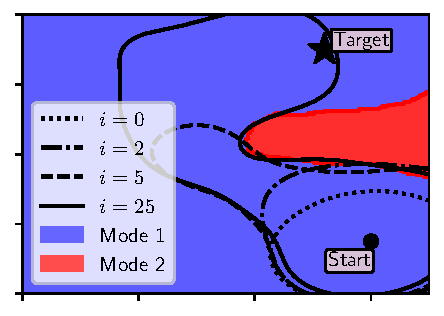
\includegraphics[width=0.92\columnwidth]{../experiments/figures/moderl_constraint_expanding.pdf}};
    %\node at (0, 0) {hey};
    \node at (3, 0.4) {\LARGE\faSkull};
    \end{tikzpicture}
    \caption{\textbf{Mode-constrained quadcopter navigation}.
    Top-down view of a quadcopter subject to
    1) an \textit{operable} dynamic mode (blue) and 2) an \textit{inoperable}, turbulent dynamic mode induced by a strong wind field (red).
    The goal is to navigate to the target whilst remaining in the \textit{operable} dynamic mode (blue).
    We achieve this by gradually expanding the $\delta\text{-mode-constrained}$ region (\cref{def-delta-mode-remaining}) at each episode $i$,
    i.e. improving our knowledge of the latent mode constraint, by training our dynamic model on new data $\mathcal{D}_{0:i}$.}
    %and reducing our un under the well-calibrated uncertainty of our dynamic model.}
    %by updating our learned dynamic model (and thus our knowledge of the latent mode constraint).}
    %However, the mode constraint is \textit{unknown a priori}.
  \label{fig-constraint-expanding}
\end{figure}
Over the last decade, reinforcement learning (RL) has become a popular paradigm for controlling dynamical systems \citep{sutton2018reinforcement,hewingLearningBased2020}.
However, RL algorithms do not typically prevent agents from entering \textit{inoperable} or \textit{undesirable} dynamic modes (\cref{def-dynamics-mode}).
This would be desirable when flying a quadcopter to a target state whilst avoiding turbulent dynamic modes,
or driving a car whilst avoiding dangerous road surfaces.
In these examples, we seek agents that can learn sample-efficiently, whilst avoiding these \textit{inoperable} or \textit{undesirable} dynamic modes.

One approach to solving this problem is to constrain the agent to a single dynamic mode during training.
However, in this mode-constrained setting, the agent does not observe the constraint.
Instead, the mode constraint is a hidden variable associated with the environment's dynamics, which are \emph{unknown a priori}.
As a result, our constraint must be simultaneously learned and enforced.

When simultaneously learning and enforcing a constraint in RL, it is impossible to guarantee constraint satisfaction.
This emphasises the need to learn sample efficiently, as each interaction with the environment could result in a constraint violation.
Further to this, constraints can prevent an agent from solving the main task (, ).
This is because they can introduce local optima that make the space of feasible policies hard to navigate.

In this paper, we present ModeRL\footnote{Code @ \href{https://github.com/aidanscannell/moderl/}{https://github.com/aidanscannell/moderl/}},
a Bayesian model-based RL algorithm, which simultaneously learns and enforces the mode constraint using
well-calibrated uncertainty estimates from a learned dynamic model.
Our main contributions are as follows:
\begin{enumerate}
\item A method for jointly inferring the mode constraint alongside the underlying dynamic modes.
\item A planning algorithm that leverages the dynamic model's well-calibrated uncertainty estimates to 1) enforce the mode constraint up to a given probability, and 2) combat local optima induced by the constraint.
\item We validate ModeRL in a simulated quadcopter navigation task.
\end{enumerate}
\section{RELATED WORK}
\label{sec:orgf0886fa}
To the best of our knowledge, there is no prior work addressing mode-constrained RL (see \cref{eq-main-problem}).
However, we can compare our method to related works, which we detail here.

\textbf{Constrained Markov decision processes (CMDPs)}
A common paradigm when considering constraints in RL is to consider CMDPs \citep{altmanConstrained1999,wachiSafeExplorationOptimization2018}.
In this setting, the agent must satisfy a set of constraints defined by additional cost functions, whose output is observed from the environment.
In contrast, the output of the constraint function is not observed in mode-constrained RL, so we cannot learn it using supervised learning.
Our work has similarities to \cite{schreiterSafe2015} as they use a Gaussian process (GP) classifier to identify safe and unsafe regions
when learning dynamic models in an active learning setting.
However, they also assume that they observe the output of their constraint function.

\textbf{Safe model predictive control (MPC)}
\cite{kollerLearningBased2018} and \cite{hewingLearningBased2020} consider safe MPC schemes which use GP dynamic models to
certify the safety of actions.
However, they do not consider environments with multimodal dynamics.
\cite{arcariDualStochasticMPC2020} is the most similar work to our own, as they consider safe stochastic MPC in dynamical systems with multiple
operating modes (synonymous to our dynamic mode in \cref{def-dynamics-mode}).
Our work differs in that we use nonparametric methods to jointly identify the mode constraint and the dynamic modes.


\textbf{Mode remaining planning}
\cite{scannellTrajectory2021} present a mode remaining trajectory optimisation algorithm that uses a learned dynamic model.
However, they do not enforce any constraints.
Further to this, they assume access to the environment \emph{a priori}.
In contrast, we consider the model-based RL setting, where we enforce the mode constraint during exploration (i.e. data collection) as well.


\textbf{Safety as stability}
In low-dimensional continuous-control problems, \cite{berkenkampSafe2017} propose to encode safety as stability via a learned dynamic model.
However, their method assumes that the environment's dynamics are Lipschitz continuous.
Although we do not provide details in this paper, we believe our method could be used to remove this assumption by constraining exploration to a subset
of the dynamics that are Lipschitz continuous.


In summary, the constraint function in mode-constrained RL is not only \emph{unknown a priori}, but its output is also not observed.
This is because it is a hidden variable associated with the environment's dynamics.
As such, it cannot be learned with supervised learning.
In the remainder of this paper, we present a model-based RL method that uses a nonparametric dynamic model to infer the mode constraint -- as a latent variable --
alongside the dynamic modes.
Importantly, it simultaneously learns and enforces the mode constraint (with high probability) during training.

\section{PROBLEM STATEMENT \label{problem-statement}}
\label{sec:orgd4a100e}
We consider environments with
states \(\state_t \in \stateDomain \subseteq \R^{\StateDim}\), actions \(\control_t \in \controlDomain \subseteq \R^{\ControlDim}\)
and \emph{multimodal}, \emph{stochastic}  transition dynamics, given by
\begin{equation}  \label{eq-dynamics}
\begin{aligned}
\state_{\timeInd+1}
%&= \dynamicsFunc(\state_\timeInd, \control_\timeInd) + \bm\epsilon_{\timeInd} \\
 &= \mode{\dynamicsFunc}(\state_\timeInd, \control_\timeInd) + \bm\epsilon_{\modeInd, \timeInd},
\quad\text{if } \modeVar(\state_{\timeInd}) = \modeInd,
\end{aligned}
\end{equation}
where the discrete mode indicator function \(\modeVar : \stateDomain \rightarrow \{1, \dots, \ModeInd\}\)
indicates which of the \(\ModeInd\) underlying dynamic modes
\(\{\mode{\latentFunc} : \mode{\stateDomain} \times \controlDomain \rightarrow \stateDomain \}_{\modeInd=1}^\ModeInd\)
and associated i.i.d. noise models \(\bm\epsilon_{\modeInd, \timeInd}\)
governs the environment at a given time step \(\timeInd\).
We refer to the output of the mode indicator function as the mode indicator variable
\(\alpha_{\timeInd} = \alpha(\state_{\timeInd}) \in \{1,\ldots,\ModeInd\}\).

\begin{definition}[dynamic mode] \label{def-dynamics-mode}
Let $\modeVar : \stateDomain \rightarrow \{0,\ldots, \ModeInd\}$ denote a function which partitions a dynamical system's $\dynamicsFunc$ state space $\stateDomain$ into
$\ModeInd$ pair-wise disjoint state domains
$\mode{\stateDomain} = \{ \state \in \stateDomain \mid \modeVar(\state) = \modeInd \}$.
Given a dynamical system comprising of $\ModeInd$ functions,
$\dynamicsFunc = \{\dynamicsFunc_{\modeInd} : \stateDomain_{\modeInd} \times \controlDomain \rightarrow \stateDomain\}_{\modeInd=1}^{\ModeInd}$,
where each function governs the system at a particular region of the state space $\stateDomain$,
we formally define a dynamic mode as,
\begin{align} \label{eq-dynamics-mode-def}
\dynamicsFunc_{\modeInd} : \stateDomain_{\modeInd} \times \controlDomain \rightarrow \stateDomain.
\end{align}
\end{definition}

Notice from \cref{def-dynamics-mode} that our dynamic modes are free to leave
their state spaces \(\mode{\stateDomain}\) and enter other modes \(\stateDomain\).

\textbf{Problem statement}
We consider controlling the stochastic system in \cref{eq-dynamics} in an episodic setting, over a horizon \(\TimeInd\).
We assume that after each episode the system is reset to a known initial state \(\state_{0}\).
We consider general deterministic policies \(\pi \in \Pi\),
which encapsulates both closed-loop policies \(\pi(\state_{\timeInd})\) and open-loop policies \(\pi(\timeInd)\).
For a known transition dynamic model \(\dynamicsFunc: \stateDomain \times \controlDomain \rightarrow \stateDomain\),
the performance of a policy \(\pi\) is the sum of rewards over the horizon, in expectation over the transition noise,
\begin{align} \label{eq-objective}
J(\pi, \dynamicsFunc) = \E_{\bm\epsilon_{0:\TimeInd}} \left[ \sum_{\timeInd=0}^{\TimeInd} \rewardFunc(\state_{\timeInd}, \control_{\timeInd}) \mid \state_0 \right].
\end{align}
The goal of our work is to find the optimal policy \(\pi^{*}\) whilst remaining in a desired dynamic mode \(\desiredMode\),
\begin{align} \label{eq-main-problem}
\argmax_{\pi \in \Pi} J(\pi, \dynamicsFunc) \quad \text{s.t. } \modeVar(\state_{\timeInd}) = \desiredMode \quad \forall \timeInd \in \{0, \ldots, \TimeInd\}.
\end{align}
Formally, a mode-constrained system is defined as follows.
\begin{definition}[mode-constrained] \label{def-mode-remaining-main}
Let $\dynamicsFunc : \stateDomain \times \controlDomain \rightarrow \stateDomain$ denote a multimodal dynamical system
and $\desiredStateDomain = \{ \state \in \stateDomain \mid \modeVar(\state) = \desiredMode \}$
denote the state domain of the desired dynamic mode $\desiredMode$.
Given an initial state $\state_0 \in \desiredStateDomain$ and a policy $\pi \in \Pi$,
the controlled system is said to be mode-constrained under the policy $\pi$ iff:
\begin{align} \label{eq-mode-remaining-def-main}
%\modeVar(\state_{\timeInd}) &\in \desiredMode \quad \forall \timeInd \in \{0, \ldots, \TimeInd\}
\dynamicsFunc(\state_{\timeInd}, \policy(\state_{\timeInd}, \timeInd)) + \epsilon_{\timeInd} &\in \stateDomain_{\desiredMode} \quad \forall \timeInd \in \{0, \ldots, \TimeInd\}
\end{align}
\end{definition}
Given that neither the underlying dynamic modes \(\{\mode{\latentFunc}\}_{\modeInd=1}^{\ModeInd}\), nor how the system
switches between them \(\modeVar\), are \emph{known a priori},
it is not possible to solve \cref{eq-main-problem} with the mode constraint in \cref{def-mode-remaining-main}.
Therefore, we relax the requirement to finding a mode-constrained policy with high probability.
We formally define a \(\delta\text{-mode-constrained}\) policy as follows.
\begin{definition}[$\delta$-mode-constrained] \label{def-delta-mode-remaining}
Let $\dynamicsFunc : \stateDomain \times \controlDomain \rightarrow \stateDomain$ denote a multimodal dynamical system
%and $\desiredMode$ a desired dynamic mode defined by its state domain $\desiredStateDomain = \{ \state \in \stateDomain \mid \modeVar(\state) = \desiredMode \}$.
and $\desiredStateDomain = \{ \state \in \stateDomain \mid \modeVar(\state) = \desiredMode \}$
denote the state domain of the desired dynamic mode $\desiredMode$.
Given an initial state $\state_0 \in \desiredStateDomain$ and $\delta \in (0,1]$,
a controlled system is said to be $\delta$-mode-constrained under the policy $\pi$ iff:
\begin{align} \label{eq-mode-remaining-def-explore}
\Pr( \forall \timeInd \in \{0,\ldots, \TimeInd \} :
%\modeVar(\state_{\timeInd}) = \desiredMode,
\dynamicsFunc(\state_{\timeInd}, \policy(\state_{\timeInd}, \timeInd)) + \epsilon_{\timeInd} &\in \stateDomain_{\desiredMode}) \geq 1 - \delta.
%\control_{\timeInd} \in \controlDomain) \geq 1 - \delta
%\Pr( \forall \timeInd \in \{0,\ldots,\TimeInd-1\} : \dynamicsFunc(\state_{\timeInd}, \policy(\state_{\timeInd}, \timeInd))
%&\in \desiredStateDomain, \policy(\state_{\timeInd}, \timeInd) \in \controlDomain) \geq 1 - \delta
\end{align}
\end{definition}
Policies satisfying this \(\delta\text{-mode-constrained}\) definition
should remain in the desired dynamic mode with probability up to \(1-\delta\).
It is worth noting that the agent would not be able to explore the environment without relaxing the
mode constraint from \cref{def-mode-remaining-main}.
Increasing \(\delta\) promotes exploration but also increases the chance of violating the mode constraint.
Intuitively, \(\delta\), which we refer to as the \emph{constraint level}, makes the mode-constrained problem
feasible, whilst still providing some level of constraint satisfaction during training.


\textbf{Initial mode remaining controller}
In robotics applications, an initial set of poor-performing controllers can normally be obtained via
simulation or domain knowledge.
We assume access to an initial data set of state transitions
\(\dataset_0 = \{(\state_{\timeInd}, \control_{\timeInd}), \state_{\timeInd+1}\}_{\timeInd=1}^{\TimeInd N_{0}}\)
from \(N_{0}\) episodes of length \(\TimeInd\).
We use it to learn a predictive dynamic model \(p(\state_{t+1} \mid \state_{\timeInd}, \action_{\timeInd}, \dataset_{0})\) which is locally accurate
around the start state \(\state_0\).
\begin{assumption} \label{}
A state transition data set has been collected
$\dataset_0 = \{(\state_{\timeInd}, \control_{\timeInd}), \state_{\timeInd+1}\}_{\timeInd=1}^{\TimeInd N_{0}}$
from an initial region of the state space $\initialStateDomain \subseteq \desiredStateDomain$, which belongs to the desired
dynamic mode $\desiredMode$ and contains the start state $\state_0 \in \initialStateDomain$.
\end{assumption}
Although such a model can be used to learn an
initial policy, it will not work outside of the initial state domain \(\initialStateDomain\) and may
not be able to find a \(\delta\text{-mode-constrained}\) policy, due to the model having high \emph{epistemic uncertainty}.
For this reason, we adopt a model-based RL strategy which incrementally explores the environment subject to a \(\delta\text{-mode constraint}\).
At each episode, it collects data and uses it to train its dynamic model.
This reduces the dynamic model's \emph{epistemic uncertainty} and expands the \(\delta\text{-mode-constrained}\) region.
See \cref{fig-constraint-expanding}.

\begin{algorithm}[!t]
\caption{ModeRL}\label{alg-mode-opt}
\begin{algorithmic}[1]
\Require{Start state $\state_0$, desired dynamic mode $\desiredMode$, initial data set $\dataset_0$, policy $\pi_{0}$, dynamic model ${p(\state_{\timeInd+1} \mid \singleInput, \dataset_{0})}$}
%\For{$i = 0, 1, \ldots $}
\For{$i  \in \{0, 1, \ldots, \text{num episodes} \}$}
    \While{not converged}
        \State Sample $N_{b}$ state transitions $\mathcal{B} \sim \dataset_{0:i}$
        \State Update dynamics using \cref{eq-lower-bound} with $\mathcal{B}$
    \EndWhile
    %\State Sample $N_{b}$ state transitions from $\dataset_{i}$ dynamics using \cref{eq-lower-bound} and $\dataset_i$
    %\State Train dynamics using \cref{eq-lower-bound} and $\dataset_i$
    \State Optimise policy $\pi_{i+1}$ using \cref{eq-joint-entropy-objective}
    %\State Collect data $\dataset_{i+1}$ from environment using $\pi_{i+1}$; add to data set ${\dataset_{0:i+1} = \dataset_{i+1} \cup \dataset_{0:i}}$
    \State Collect data $\dataset_{i+1}$ using $\pi_{i+1}$
    \State Update agent's data set ${\dataset_{0:i+1} = \dataset_{i+1} \cup \dataset_{0:i}}$
\EndFor
\end{algorithmic}
\end{algorithm}

\section{MODE-CONSTRAINED MODEL-BASED RL \label{sec-mode-optimisation}}
\label{sec:org788d667}
We propose to solve the mode-constrained RL problem in \cref{eq-main-problem} by synergising model learning and planning in a
model-based RL algorithm we name mode-constrained model-based reinforcement learning (ModeRL).
Our approach is detailed in \cref{alg-mode-opt}.
\subsection{Probabilistic Dynamic Model}
\label{sec:org36bd6dc}

ModeRL learns a single-step dynamic model and we adopt the delta state formulation to regularise the predictive distribution.
We denote a state difference output as \(\singleOutput = \state_{t+1} - \state_{t}\) and the set of all state difference outputs as  \(\allOutput\).
We further denote a state-action input as \(\singleInput = (\state_{\timeInd}, \action_{\timeInd})\), the set of all state-action inputs
as \(\allInput\), the set of all state inputs as \(\allState\) and the state transition data set at episode \(i\) as \(\dataset_{0:i}\).

The main goal of our dynamic model is to jointly infer the mode constraint along with the underlying dynamic modes.
In particular, we would like our model to,
\begin{enumerate}
\item Formulate a prior over the mode constraint where we can encode prior knowledge, potentially enabling ModeRL to find a policy without ever violating the mode constraint.
In practice, encoding prior knowledge allows us to exploit Bayesian interpolation (, a) to reduce the number of constraint violations during training.
\item Disentangle the sources of uncertainty in the mode constraint so that ModeRL can escape local optima induced by the constraint (via intrinsic exploration with the mode constraint's \emph{epistemic uncertainty}).
\end{enumerate}

\textbf{Marginal likelihood}
Mixtures of Gaussian process experts (MoGPE) models are a natural choice for modelling multimodal systems as they automatically infer the assignment of observations to
dynamic modes (experts).
Let us start by introducing the MoGPE marginal likelihood,
\begin{align} \label{eq-np-moe-marginal-likelihood-main}
%\moeEvidence
\evidence
%&= \sum_{\allModeVar} \npmoeGatingPosterior \npmoeExpertPosterior  \\
&= \sum_{\allModeVar}
\underbrace{p \left(\bm\modeVar \mid \allState \right)}_{\text{gating network}}
\bigg[ \prod_{\modeInd=1}^\ModeInd
\underbrace{p\left(\allOutputK \mid \allInputK, \expertParamsK \right)}_{\text{dynamic mode } \modeInd}
\bigg]
\end{align}
where \(\allInputK\) denotes the set of \(\NumData_{\modeInd}\) inputs assigned to dynamic mode \(\modeInd\), i.e.
\(\allInputK = \{\singleInput \in \allInput \mid \modeVar(\state_{\timeInd}) = \modeInd\}\).
Similarly for the outputs we have \(\allOutputK = \{\singleOutput \in \allOutput \mid \modeVar(\state_{\timeInd+1}) = \modeInd\}\).
Note that there is a joint distribution corresponding to every possible combination of assignments
of observations to dynamic modes.
Hence, \cref{eq-np-moe-marginal-likelihood-main} is a sum over exponentially many (\(\ModeInd^{\NumData}\)) sets of assignments,
where \(\allModeVar = \{\modeVar_1, \ldots, \modeVar_\NumData \}\) represents a set of assignments for all observations.
This distribution factors into the product over modes, where each mode models the joint Gaussian distribution
over the observations assigned to it.

\textbf{Learning the mode constraint}
The gating network indicates which dynamic mode governs the system at a given state input.
It is of particular importance in our work as we use it to represent our mode constraint.
Motivated by synergising model learning and planning, we formulate our gating network using input-dependent functions --
known as gating functions -- and place GP priors over them.
In \cref{sec-planning} we exploit the disentangled \emph{epistemic uncertainty} represented in our
GP-based gating network to help ModeRL escape local optima induced by the mode constraint.
Similar to \cite{trespMixtures2000a}, our gating network resembles a GP classification model,
\begin{align} \label{eq-prob-mass}
\npmoeGatingPosterior &= \E_{\underbrace{p(\GatingFunc(\allState)) }_{\text{GP prior(s)}}} \bigg[ \prod_{\numData=1}^{\NumData}
\underbrace{p \left(\modeVar_{\timeInd} \mid \GatingFunc(\state_{\timeInd}) \right)}_{\text{classification likelihood}} \bigg]
%\allModeVar \mid \GatingFunc(\allInput) &\sim \prod_{\numData=1}^{\NumData} \text{Cat} \left( \text{softmax}   \left(\GatingFunc(\singleInput)\right) \right) \\
%\GatingFunc(\allInput) &\sim \prod_{\modeInd=1}^\ModeInd \mathcal{N}\left( \gatingMeanFunc(\allInput), \gatingCovFunc(\allInput, \allInput) \right),
\end{align}
where \(p\left(\modeVar_{\timeInd} \mid \GatingFunc(\state_{\timeInd})\right)\) represents a classification likelihood parameterised by \(\ModeInd\) gating
functions \(\GatingFunc: \stateDomain \rightarrow \mathbb{R}^{\ModeInd}\).
We use a Bernoulli likelihood when \(\ModeInd=2\) and a softmax when \(\ModeInd>2\).
We place GP priors on each of the gating functions
\(p(\GatingFunc(\allInput)) = \prod_{\modeInd=1}^\ModeInd \mathcal{N}\left( p(\mode{\gatingFunc}(\allInput) \mid \gatingMeanFunc(\allInput), \gatingCovFunc(\allInput, \allInput) \right)\),
where \(\gatingMeanFunc(\cdot)\) and \(\gatingCovFunc(\cdot,\cdot)\) represent the mean and covariance functions
associated with the \(\modeInd^\text{th}\) gating function \(\mode{\gatingFunc}\).
In our gating network formulation, the GP posteriors represent the mode constraint's \emph{epistemic uncertainty}.
\newline

\textbf{Dynamic modes}
We model the underlying dynamic modes as independent GP regression models,
\begin{align}
\underbrace{p\left(\allOutputK \mid \allInputK \right)}_{\text{dynamic mode } \modeInd}
&= \underbrace{\E_{p(\mode{\latentFunc}(\allInputK))}}_{\text{GP prior}} \bigg[
\prod_{\numData=1}^{\NumData_{\modeInd}}
\underbrace{p\left(\singleOutput \mid \mode{\latentFunc}(\singleInput)\right)}_{\text{Gaussian likelihood}}
\bigg], \nonumber
%\allOutputK \mid \mode{\latentFunc}(\allInputK) &\sim \prod_{\numData=1}^{\NumData_{\modeInd}} \mathcal{N}\left( \singleOutput \mid \mode{f}(\singleInput), \mode{\noiseVar}^2 \right) \label{eq-expert-likelihood} \\
%\mode{\latentFunc}(\allInputK) &\sim \mathcal{N}\left( \expertMeanFunc(\allInputK), \expertCovFunc(\allInputK, \allInputK) \right), \label{eq-expert-prior}
\end{align}
where each mode's GP prior is given by
\(p(\mode{\latentFunc}(\allInputK)) = \mathcal{N} \left( \mode{\latentFunc}(\allInputK) \mid \expertMeanFunc(\allInputK), \expertCovFunc(\allInputK, \allInputK) \right)\)
with \(\expertMeanFunc(\cdot)\) and \(\expertCovFunc(\cdot, \cdot)\) representing the mean and
covariance functions associated with the \(\modeInd^{\text{th}}\) mode's GP prior respectively.
Note that as the assignment of observations to modes is \emph{not known a priori}, we must infer the assignments from observations.
In our model, each dynamic mode's Gaussian likelihood represents the mode's \emph{aleatoric uncertainty} (the transition noise in this case)
whilst each mode's GP posterior represents the mode's \emph{epistemic uncertainty}.

\subsection{Dynamic Model Learning \label{sec-dynamics-learning}}
\label{sec:org2ba2001}
Performing Bayesian inference in our dynamic model involves finding the posterior over the latent variables
\(p(\{\latentFunc(\allInput)\}_{\modeInd=1}^{\ModeInd}, \GatingFunc(\allState) \mid \dataset_{0:i})\),
which requires calculating the marginal likelihood in \cref{eq-np-moe-marginal-likelihood-main}.
As such, exact inference in our model is intractable due to the marginalisation over the set of mode
indicator variables. For this reason, we resort to a variational approximation.



Following the approach by \cite{titsiasVariational2009}, we augment the probability space
with a set of inducing variables for each GP.
However, instead of collapsing these inducing variables, we
represent them as variational distributions and use them to lower bound the marginal likelihood, similar to
\cite{hensmanGaussian2013,hensmanScalable2015}.
\cref{fig-graphical-model-sparse} shows the graphical model of the augmented joint probability space.

\textbf{Augmented dynamic modes}
We sidestep the hard assignment of observations to modes by augmenting each dynamics GP with a set
of \(\NumInducing_{\mode{\latentFunc}}\) separate independent inducing points,
\begin{align} \label{eq-experts-inducing-prior}
\expertInducingPrior
&=  \mathcal{N}\left( \expertInducingOutput \mid
\expertMeanFunc(\expertInducingInput),
\expertCovFunc(\expertInducingInput, \expertInducingInput) \right).
\end{align}
Introducing separate inducing points from each mode's GP can loosely be seen as "partitioning"
the observations between modes.
However, as the assignment of observations to modes is \emph{not known a priori}, the inducing inputs
\(\expertInducingInput\) and variables \(\expertInducingOutput\), must be inferred from observations.

\textbf{Augmented gating network}
We follow a similar approach for the gating network and augment each gating function GP with a
set of \(\NumInducing_{\mode{\gatingFunc}}\) inducing points,
\begin{align} \label{eq-gatings-inducing-prior}
\gatingInducingPrior
&= \mathcal{N}\left( \gatingInducingOutput \mid
\gatingMeanFunc(\gatingInducingInput),
\gatingCovFunc(\gatingInducingInput, \gatingInducingInput) \right).
\end{align}
The distribution over all gating functions is denoted \(\gatingsInducingPrior =\prod_{\modeInd=1}^\ModeInd \gatingInducingPrior\).
In contrast to the dynamic modes, the gating function GPs share inducing inputs \(\gatingInducingInput\).

\textbf{Marginal likelihood}
We use these inducing points to approximate the true marginal likelihood with,
%\small
\begin{align} \label{eq-augmented-marginal-likelihood-main}
\evidence &\approx
\E_{\gatingsInducingPrior \expertsInducingPrior} \bigg[  \\
&\prod_{\numData=1}^{\NumData} \sum_{\modeInd=1}^{\ModeInd} \singleGatingGivenInducing  \singleExpertGivenInducing \bigg], \nonumber
\end{align}
%\normalsize
where the conditional distributions \(\singleExpertGivenInducing\) and \(\singleGatingGivenInducing\)
follow from standard sparse GP methodologies.
See \cref{eq-sparse-gp-methodologies-gating,eq-sparse-gp-methodologies} in \cref{sec-sparse-approximations}.
Importantly, the factorisation over observations is outside of the marginalisation over the mode indicator variable, i.e.
the mode indicator variable can be marginalised for each data point separately.
This is not usually the case for MoGPE methods.
Our approximation assumes that the inducing variables,
\(\{\expertInducingOutput\}_{\modeInd=1}^\ModeInd\), are
a sufficient statistic for their associated latent function values,
\(\{\mode{\latentFunc}(\allInputK) \}_{\modeInd=1}^\ModeInd\)
and the set of assignments \(\allModeVar\).
It becomes exact when each mode's inducing points represent the true data partition
\(\{\expertInducingInput, \expertInducingOutput\}_{\modeInd=1}^{\ModeInd} = \{\allInputK, \mode{\latentFunc}(\allInputK)\}_{\modeInd=1}^{\ModeInd}\).

\textbf{Evidence lower bound (ELBO)}
Following a similar approach to \cite{hensmanGaussian2013,hensmanScalable2015},
we lower bound \cref{eq-augmented-marginal-likelihood-main},
%\small
\begin{align} \label{eq-lower-bound}
\mathcal{L}(\{\mode{\mathbf{m}}, &\mode{\mathbf{L}}, \mode{\hat{\mathbf{m}}}, \mode{\hat{\mathbf{L}}}, \expertInducingInput\}_{\modeInd=1}^{\ModeInd}, \gatingInducingInput) =
%\sum_{(\singleInput, \singleOutput) \in \dataset_{0:i}}
\sum_{\timeInd=1}^{\NumData}
\E_{\gatingsVariational \expertsInducingVariational}
\bigg[ \nonumber \\
&\text{log} \sum_{\modeInd=1}^{\ModeInd} \singleGatingLikelihood  \singleExpertGivenInducing \bigg] \nonumber \\
&- \expertsKL \nonumber \\
&- \gatingsKL
\end{align}
%\normalsize

where the dynamic mode's variational posterior is given by
\(\expertsInducingVariational = \prod_{\modeInd=1}^{\ModeInd} \mathcal{N}\left(\expertInducingOutput \mid \mode{\mathbf{m}}, \mode{\mathbf{L}} \mode{\mathbf{L}}^{T} \right)\)
and the gating network's variational posterior is given by
\(\gatingsVariational = \prod_{\modeInd=1}^{\ModeInd} \int \singleLatentGatingGivenInducing \mathcal{N}\left(\gatingInducingOutput \mid \mode{\hat{\mathbf{m}}}, \mode{\hat{\mathbf{L}}}\mode{\hat{\mathbf{L}}}^{T} \right) \text{d}\GatingFunc(\gatingInducingInput)\).

\textbf{Optimisation}
The bound in \cref{eq-lower-bound} induces a local factorisation over observations and has a set of global variables
-- the necessary conditions to perform stochastic variational inference (SVI) (, a) on
\(\expertsInducingVariational\) and \(\gatingsInducingVariational\), i.e.
optimise \(\{\mode{\mathbf{m}}, \mode{\mathbf{L}}, \mode{\hat{\mathbf{m}}}, \mode{\hat{\mathbf{L}}}\}_{\modeInd=1}^{\ModeInd}\).
We treat the inducing inputs \(\gatingInducingInput,\{\expertInducingInput\}_{\modeInd=1}^{\ModeInd}\),
kernel hyperparameters and noise variances, as
variational hyperparameters and optimise them alongside the variational parameters, using Adam \citep{kingmaAdam2017}.
We use mini-batches and approximate the expectations over the log-likelihood using Monte Carlo samples.

Our approach can loosely be viewed as parameterising the nonparametric model in \cref{eq-np-moe-marginal-likelihood-main} to obtain a desirable
factorisation for 1) constructing a GP-based gating network and 2) deriving an ELBO that can be optimised with stochastic gradient methods.
Importantly, our approach still captures the complex dependencies between the gating network and dynamic modes.


\textbf{Predictions}
Given our variational approximation, we make predictions at a new input \(\singleInput\) with,
\small
\begin{equation} \label{eq-dynamics-approx-predictions}
\begin{aligned}
p(\mode{\latentFunc}(\singleInput) \mid \singleInput, \dataset_{0:i})
&\approx \int p(\mode{\latentFunc}(\singleInput) \mid \mode{\latentFunc}(\expertInducingInput))
q(\mode{\latentFunc}(\expertInducingInput)) \text{d} \mode{\latentFunc}(\expertInducingInput), \nonumber \\
p(\mode{\gatingFunc}(\state_{\timeInd}) \mid \state_{\timeInd}, \dataset_{0:i})
&\approx \int p(\mode{\gatingFunc}(\state_{\timeInd}) \mid \mode{\gatingFunc}(\gatingInducingInput))
q(\mode{\gatingFunc}(\gatingInducingInput))
\text{d} \mode{\gatingFunc}(\gatingInducingInput). \nonumber
\end{aligned}
\end{equation}
\normalsize
See \cref{eq--variational-posteriors-functional-gating,eq--variational-posteriors-functional-experts} in \cref{sec-sparse-approximations}.

\begin{figure*}[!t]
  \centering
  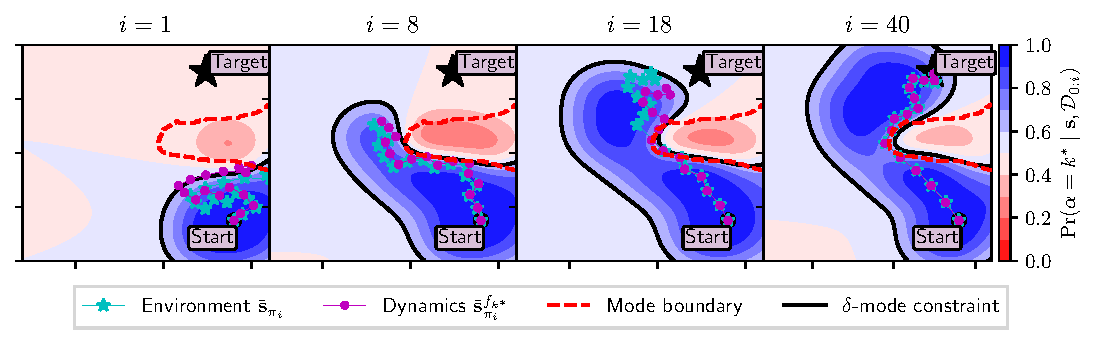
\includegraphics[width=0.91\textwidth]{../experiments/figures/moderl_four_iterations_in_row.pdf}
  \caption{Visualisation of four episodes $i$ of ModeRL in the quadcopter navigation task from
  \cref{fig-problem-statement}.
  The goal is to navigate to the black star, whilst avoiding the turbulent dynamic mode (dashed red line).
  The contour plots indicate the agent's belief of being in the desired dynamic mode $\Pr(\modeVar=\desiredMode \mid \state, \dataset_{0:i})$ at each episode,
  i.e. after training on $\dataset_{0:i}$.
  The black lines show the $\delta\text{-mode constraint}$ (see \cref{eq-expected-constraint}) expanding during training.
  At each episode $i$ we roll out the policy in the desired dynamic mode's GP (magenta) as well as the in the environment (cyan). Experiments used an exponentially decaying schedule on $\delta$ to tighten the mode constraint during training.}
  %The environment trajectories (cyan) deviate from the dynamics trajectories (magenta) when the trajectories leave the desired dynamic mode.}
  \label{fig-joint-entropy-four-episodes}
\end{figure*}
\subsection{Planning \label{sec-planning}}
\label{sec:org9ca74a8}
We now detail our planning algorithm which leverages the latent structure of our dynamic model to:
\begin{enumerate}
\item Enforce the mode constraint with high probability,
\item Escape local optima induced by the mode constraint, by targeting exploration where the agent has high \emph{epistemic uncertainty} in its belief of the mode constraint.
\end{enumerate}

\textbf{Multi-step predictions with dynamic model}
Let us first observe that if the controlled system satisfies the mode constraint, the system will be fully
governed by the desired dynamic mode \(\dynamicsFunc_{\desiredMode}\).
We leverage this observation and simplify making multi-step predictions by using only the desired
dynamic mode \(\dynamicsFunc_{\desiredMode}\).
This enables us to approximate the GP dynamics integration in closed form using moment matching
(, a, , a, , a).
See \cref{sec-moment-matching} for more details.
This approximation has been shown to work well in RL
contexts (, a, , a, , a, , a, , a).

\textbf{Objective}
Given this approach for making multi-step predictions, we use \cref{def-delta-mode-remaining}
to formulate a relaxed version of the mode-constrained problem in \cref{eq-main-problem},
\begin{subequations} \label{eq-greedy-objective}
\begin{align}
%&\pi_{\text{greedy}}=
&\argmax_{\pi \in \Pi}
\underbrace{\E_{p(\dynamicsFunc_{\desiredMode} \mid \dataset_{0:i})} \left[ J(\pi, \dynamicsFunc_{\desiredMode}) \right]}_{\text{greedy exploitation}},
\label{eq-greedy-objective-term}
\\
&\text{s.t. }
\underbrace{\Pr(\modeVar_{\timeInd} = \desiredMode \mid \state_{0}, \action_{0:t}, \dataset_{0:i})
\geq 1-\delta}_{\delta\text{-mode constraint}}, \quad \forall \timeInd \label{eq-expected-constraint}.
%\underbrace{\E_{\dynamicsFunc_{\desiredMode} \sim p(\dynamicsFunc_{\desiredMode} \mid \dataset_{0:i})}
%\left[ \Pr(\modeVar_{\timeInd} = \desiredMode \mid \state_{\timeInd}) \right]
%\geq 1-\delta}_{\delta\text{-mode constraint}}, \quad \forall \timeInd \label{eq-expected-constraint},
\end{align}
\end{subequations}
The expectation is taken over the desired dynamic mode's \(\dynamicsFunc_{\desiredMode}\) GP.
Note that the expected objective in \cref{eq-greedy-objective-term}, which we refer to as greedy exploitation, is widely adopted.
For example, in PILCO (, a), PETS (, a) and GP-MPC (, a).
We calculate the \(\delta\text{-mode constraint}\) in \cref{eq-expected-constraint} as,
\begin{align} \label{eq--delta-mode-constraint-approx}
&\Pr (\modeVar_{\timeInd}=\desiredMode \mid \state_{0}, \action_{0:\timeInd}, \dataset_{0:i}) =   \\
\ &\int \Pr(\modeVar_{\timeInd}=\desiredMode \mid \gatingFunc(\state_{\timeInd}))
\underbrace{p(\gatingFunc(\state_{\timeInd}) \mid \state_{0}, \action_{0:\timeInd}, \dataset_{0:i})}_{\text{gating posterior at \timeInd}}
\text{d} \gatingFunc(\state_{\timeInd}), \nonumber
\end{align}
where \(\Pr(\modeVar_{\timeInd}=\desiredMode \mid \gatingFunc(\state_{\timeInd}))\) resembles a classification likelihood (see \cref{sec-gating-network-app}).
We approximate the gating function posterior predicted \(\timeInd\) steps into the future,
\begin{align}
&\underbrace{p(\gatingFunc(\state_{\timeInd}) \mid \state_{0}, \action_{0:\timeInd}, \dataset_{0:i})}_{\text{gating posterior at \timeInd}}
= \nonumber \\
&\quad \int
\underbrace{p\left(\gatingFunc(\state_{\timeInd}) \mid \state_{\timeInd}, \dataset_{0:i} \right)}_{\text{gating posterior}}
\underbrace{p(\state_{\timeInd} \mid \state_{0}, \action_{0:\timeInd-1}, \mathcal{D}_{0:i})}_{\text{dynamics posterior}} \text{d} \state_{\timeInd},
\end{align}
by propagating the state's uncertainty using moment matching (see \cref{sec-moment-matching}),
where the state distribution
\({p(\state_{\timeInd} \mid \state_{0}, \action_{0:\timeInd-1}, \mathcal{D}_{0:i})}\) is obtained by cascading single-step predictions using
moment matching (see \cref{sec-moment-matching}).
Importantly, the \(\delta\text{-mode constraint}\) considers 1) both the \emph{epistemic} and \emph{aleatoric uncertainties} in the desired dynamic mode
and 2) the \emph{epistemic uncertainty} in the gating network.
This ensures that the controlled system is \(\delta\text{-mode-constrained}\) (\cref{def-delta-mode-remaining}) under the uncertainty of the learned dynamic model.
Intuitively, it will remain where the dynamic model's \emph{uncertainty} is low because the expectation results in lower probabilities for more uncertain states.

\begin{figure*}[!t]
    \centering
    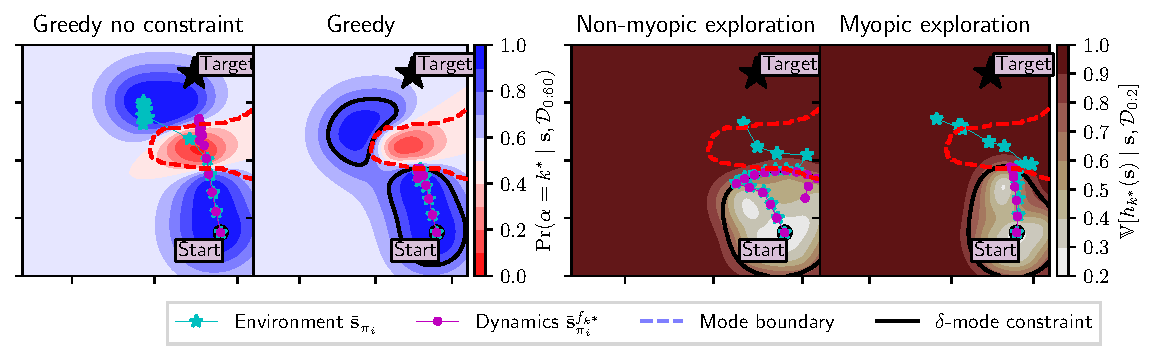
\includegraphics[width=0.88\textwidth]{../experiments/figures/greedy_and_myopic_comparisons.pdf}
  \caption{(Left) show trajectories found by the greedy exploitation strategy in \cref{eq-greedy-objective}, with and without
  the $\delta\text{-mode constraint}$ (black line).
  (Right) shows trajectories found by our strategy in \cref{eq-joint-entropy-objective} when using our
  non-myopic exploration term $\mathcal{H}[\gatingFunc_{\desiredMode}(\stateTraj) \mid \stateTraj, \dataset_{0}]$,
  compared to using the myopic exploration term
  $\frac{1}{\TimeInd}\sum_{\timeInd=1}^{\TimeInd} \mathcal{H}[\gatingFunc_{\desiredMode}(\state_{\timeInd}) \mid \state_{\timeInd}, \dataset_{0}]$.
  We overlay the trajectories on the GP posterior variance associated with desired mode's gating function
  $\mathbb{V}[\gatingFunc_{\desiredMode}(\state) \mid \state, \dataset_{0}]$ at episode $i=0$.}
  \label{fig-ablations}
\end{figure*}
\textbf{Exploration}
In our experiments, the constraint in \cref{eq-expected-constraint} hinders exploration and prevents the agent from solving the task.
This can be seen in the second from the left plot in \cref{fig-ablations}, where the mode constraint has induced a local
optimum and stopped the agent from reaching the target state.
We name the approach in \cref{eq-greedy-objective} the greedy constrained strategy.
We propose to overcome the issue of local optima induced by the mode constraint,
by targeting exploration where the agent has high \emph{epistemic uncertainty} in the mode constraint.
We do this by augmenting our objective with an intrinsic exploration term that encourages the agent to explore where its gating network is \emph{uncertain}.
We use the entropy of the desired mode's gating function \(\gatingFunc_{\desiredMode}\) over a
trajectory \(\stateTraj=\{\state_{0},\ldots, \state_{\TimeInd} \}\) as our intrinsic exploration term.
This leads to our strategy taking the form,
\begin{subequations} \label{eq-joint-entropy-objective}
%\small
\begin{align}
%&\pi_{\text{entropy}}=
&\argmax_{\pi \in \Pi}
\underbrace{\E_{p(\dynamicsFunc_{\desiredMode} \mid \dataset_{0:i})} \left[ J(\pi, \dynamicsFunc_{\desiredMode}) \right]}_{\text{greedy exploitation}} +
\beta\underbrace{\mathcal{H} \left[
\desiredGatingFunction(\stateTraj) \mid \stateTraj, \dataset_{0:i} \right]}_{\text{exploration}} \\
%&\text{s.t. } \underbrace{\E_{\dynamicsFunc_{\desiredMode} \sim p(\dynamicsFunc_{\desiredMode} \mid \dataset_{0:i})} \left[ \Pr(\modeVar_{\timeInd} = \desiredMode \mid \state_{\timeInd}) \right]
%\geq 1-\delta}_{\delta \text{ mode constraint}} \quad \forall \timeInd.
&\text{s.t. } \underbrace{ \Pr \left(\modeVar_{\timeInd} = \desiredMode \mid \state_{0}, \action_{0:\timeInd}, \mathcal{D}_{0:i} \right)
\geq 1-\delta}_{\delta\text{-mode constraint}} \quad \forall \timeInd.
%\in \{ 0, \ldots, \TimeInd \} \nonumber
\end{align}
\end{subequations}
%\normalsize
where \(\beta\) is a hyperparameter that sets the level of exploration.
Intuitively, the entropy term should enable the agent to escape local optima induced by the mode constraint as it
encourages the agent to explore away from regions of the mode constraint that it has already observed.
This is because the gating network's \emph{epistemic uncertainty} will be low where it has observed the environment.

\textbf{Epistemic vs aleatoric uncertainty}
When adopting this approach, it is extremely important to disentangle the gating network's \emph{epistemic uncertainty} from its \emph{aleatoric uncertainty}.
For example, what is the meaning of the agent's belief in the mode indicator variable
tending to a uniform distribution i.e. \(\Pr(\modeVar=\modeInd \mid \state, \dataset_{0:i})=\frac{1}{\ModeInd}\)?
Does it mean that the agent has not observed the environment near \(\state\) (high \emph{epistemic uncertainty}), or
that it has observed the environment near \(\state\) but is still uncertain which mode governs the dynamics (high \emph{aleatoric uncertainty})?
We show the importance of disentangling these sources of uncertainty in our experiments.
This motivated our GP-based gating network in the MoGPE dynamic model, as it principally
disentangles the sources of uncertainty over \(\alpha\), by representing the \emph{epistemic uncertainty} in the gating network's GPs.


\textbf{Non-myopic exploration}
Further to providing a principled approach for disentangling sources of uncertainty, our GP-based gating network enables us to deploy a non-myopic exploration strategy.
That is, we are able to steer the agent along a trajectory that will maximise uncertainty reduction over the entire trajectory,
by considering the joint entropy over a trajectory \(\mathcal{H}[\gatingFunc_{\desiredMode}(\stateTraj) \mid \stateTraj, \dataset_{0}]\).
In contrast, myopic exploration considers uncertainty reduction of each state independently without considering the influence of other states in the trajectory,
e.g. \(\frac{1}{\TimeInd}\sum_{\timeInd=0}^{\TimeInd}\mathcal{H}[\gatingFunc_{\desiredMode}(\state_{\timeInd}) \mid \state_{\timeInd}, \dataset_{0}]\).

\textbf{Trajectory optimisation}
We use an open-loop trajectory optimisation policy because it naturally handles the \(\delta\text{-mode}\) constraint
in \cref{eq-joint-entropy-objective}.
Given a start state \(\state_{0}\), ModeRL finds the action sequence \(\bar{\action} = \{\action_{0},\ldots,\action_{\TimeInd-1}\}\) solving the following optimal control problem,
\begin{subequations} \label{eq-trajectory-optimisation}
\begin{align}
&\argmax_{\action_{0}, \ldots, \action_{\TimeInd-1}}
\underbrace{\E_{p(\dynamicsFunc_{\desiredMode} \mid \dataset_{0:i})} \left[ J(\pi, \dynamicsFunc_{\desiredMode}) \right]}_{\text{greedy exploitation}}
+ \beta \underbrace{\ln \left( | (2\pi e) \bm\Sigma_{\desiredMode}(\bar{\state}, \bar{\state}) | \right)}_{\text{exploration}} \\
%+ \beta\underbrace{\mathcal{H} \left[
%\desiredGatingFunction(\stateTraj) \mid \stateTraj, \dataset_{0:i} \right]}_{\text{exploration}} \\
&\text{s.t. } \underbrace{ \Pr \left(\modeVar_{\timeInd} = \desiredMode \mid \state_{0}, \action_{0:t}, \mathcal{D}_{0:i} \right)
\geq 1-\delta}_{\delta\text{-mode constraint}} \quad \forall \timeInd \in \{0,\ldots, \TimeInd\}, \label{eq-constraint-approx}
\end{align}
\end{subequations}
where the greedy exploitation term is an expectation over the state distribution obtained from making multi-step predictions
in the desired dynamic mode's GP using moment-matching, see \cref{eq-moment-matching-system-function}.
\(\bm\Sigma^{2}_{\desiredMode}(\bar{\state},\bar{\state})\) is the predictive covariance of the desired mode's
gating function posterior over the trajectory \(\bar{\state}\), given in \cref{eq-joint-gating-covariance}.
It is worth noting a closed-loop policy can be obtained using MPC.
However, this would require our algorithm to be made faster,
for example, via locally linear dynamics approximations.
Alternatively, a closed-loop policy could be learned, for example, via guided policy search (, a).

\begin{figure*}[t]
    \centering
    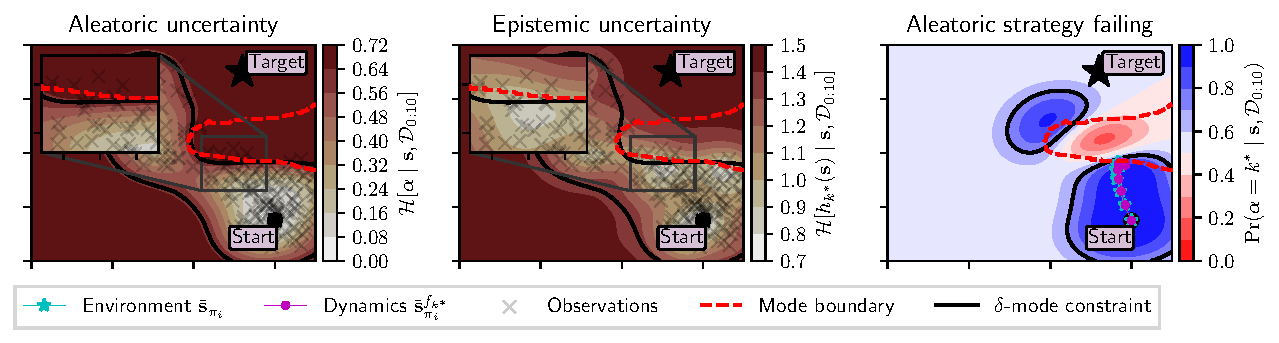
\includegraphics[width=0.95\textwidth]{../experiments/figures/uncertainty_comparison.pdf}
    \caption{\textbf{Epistemic vs aleatoric uncertainty} Illustration of the shortcomings of using the entropy of the mode indicator variable
    (\textit{aleatoric uncertainty}) for exploration.
    (Left) shows that the entropy of the mode indicator variable $\mathcal{H}[\modeVar \mid \state, \dataset_{0:10}]$ (\textit{aleatoric uncertainty}) at a region of the mode boundary
    which has been observed (black crosses), is high (red), even though we have observed the environment at these states.
    In contrast, (middle) shows that the entropy of the desired mode's gating function $\mathcal{H}[\gatingFunc_{\desiredMode}(\state) \mid \state, \dataset_{0:10}]$
    (\textit{epistemic uncertainty}) is low (white).
    (Right) visualises ModeRL converging to a local optimum when we replace the intrinsic exploration term in \cref{eq-joint-entropy-objective} with the
    entropy of the mode indicator variable.}
    \label{fig-uncertainty-comparison}
\end{figure*}

\section{EXPERIMENTAL RESULTS}
\label{sec:org628d74d}
We test ModeRL on a 2D quadcopter navigation example, where the goal is to navigate to a target state \(\state_{f}\), whilst avoiding a turbulent dynamic mode.
See \cref{illustrative_example} for a schematic of the environment and details of the problem.
Our experiments seek to answer the following questions:
\begin{enumerate}
\item Why does the greedy exploitation strategy in \cref{eq-greedy-objective} fail to solve the mode-constrained problem in \cref{eq-main-problem}?
\item Does ModeRL, our strategy in \cref{eq-joint-entropy-objective}, solve the mode-constrained problem in \cref{eq-main-problem}?
\item Is it important to disentangle the sources of uncertainty in the mode constraint?
\item Does our non-myopic exploration strategy help?
\item How does the constraint level \(\delta\) influence training?
\end{enumerate}


To evaluate ModeRL, we compare against the greedy baseline strategy in \cref{eq-greedy-objective}
(whose objective is used by PILCO (, a), PETS (, a), GP-MPC (, a)),
both with and without the \(\delta\text{-mode}\) constraint in \cref{eq-expected-constraint}.
Our experiments' configurations are detailed in \cref{sec-experiment-configuration}.

Given the quadratic reward function in \cref{eq-reward-func} our objective has closed form.
Further to this, we use two dynamic modes so our \(\delta\text{-mode}\) constraint also has a closed form.
At each episode, we then solve,
\begin{subequations} \label{eq-explorative-traj-opt}
\begin{align}
%\pi(\timeInd)
&\argmax_{\action_{0}, \ldots, \action_{\TimeInd-1}}
\underbrace{- \|\bm\mu^{\text{MM}}_{\state_{\TimeInd}} - \targetState \|_{\mathbf{H}}
+\text{Tr} \left(\mathbf{H} \bm\Sigma^{\text{MM}}_{\state_{\TimeInd}} \right)}_{\text{terminal state reward}} \nonumber \\
&\quad\quad - \sum_{\timeInd=0}^{\TimeInd-1} \big(
\underbrace{\|\bm\mu^{\text{MM}}_{\state_{\timeInd}} - \targetState \|_{\mathbf{Q}}
-\text{Tr} \left(\mathbf{Q} \bm\Sigma^{\text{MM}}_{\state_{\timeInd}} \right)}_{\text{state difference reward}}
+ \underbrace{\|\control_{\timeInd} \|_{\mathbf{R}}}_{\text{control reward}}
\big)
%- \underbrace{\control_{\timeInd}^{\TimeInd} \mathbf{R} \control_{\timeInd}}_{\text{control reward}}
\nonumber \\
&\quad\quad + \beta \underbrace{\ln \left( | (2\pi e) \bm\Sigma^2_{\desiredMode}(\bar{\state}, \bar{\state}) | \right)}_{\text{joint gating entropy}} \\
&\quad \text{s.t. } \underbrace{\Phi \bigg( \frac{\bm\mu_{\desiredMode}(\state_{\timeInd})}{\sqrt{1+ \bm\Sigma^2_{\desiredMode}(\state_{\timeInd}, \state_{\timeInd})}} \bigg)
\geq 1-\delta}_{\delta\text{-mode constraint}} \quad \forall \timeInd \in \{ 0, \ldots, \TimeInd \}
\end{align}
\end{subequations}
where \(\bm\mu_{\desiredMode}(\state_{\timeInd})\) and \(\bm\Sigma^{2}_{\desiredMode}(\state_{\timeInd},\state_{\timeInd})\)
are the predictive mean and covariance
of the desired mode's gating function posterior at
\(\state_{\timeInd}\), given in \cref{eq-gating-predictive-eqns,eq-joint-gating-covariance}.
\(\bm\mu^{\text{MM}}_{\state_{\timeInd}}\) and
\(\bm\Sigma^{\text{MM}}_{\state_{t}}\) are the mean and covariance of the state predicted \(\timeInd\) steps into the future
\(p(\state_{\timeInd} \mid \state_{0}, \action_{0:\timeInd-1}, \mathcal{D}_{0:i})\), obtained
by cascading single-step predictions through the desired dynamic mode's GP with moment matching, given in \cref{eq-moment-matching-system-function}.
\(\mathbf{H}\) and \(\mathbf{Q}\) are user-defined, real symmetric positive semi-definite
weight matrices and \(\mathbf{R}\) is a user-defined, positive definite weight matrix.
We solve  \cref{eq-explorative-traj-opt}
using sequential least squares quadratic programming (SLSQP) in SciPy (, a),
using the TensorFlow (, a) wrapper provided by GPflow (, a).


\textbf{Why does greedy exploitation fail?}
Using the greedy strategy without the mode constraint results in the optimisation finding trajectories that leave the desired dynamic mode.
This is illustrated in \cref{fig-ablations} (left), which shows the unconstrained greedy strategy converged to a solution navigating
straight to the target state.
As a result, the trajectory leaves the desired dynamic mode and passes through the turbulent dynamic mode.
This is expected as the strategy is not aware of the turbulent dynamic mode.
In contrast, the constrained greedy strategy in \cref{fig-ablations} (second left), does not leave the desired dynamic mode.
However, the optimisation does not converge to the global optimum, i.e. the trajectory does not navigate to the target state \(\targetState\).
Instead, it gets stuck at the mode boundary, i.e. a local optimum.

\textbf{Does our uncertainty-guided exploration work?}
The failure of the greedy strategy motivated our nonparametric dynamic model which learns the \(\delta\text{-mode}\) constraint -- as a latent variable -- alongside the
dynamic modes.
Importantly, this enabled ModeRL (in \cref{eq-joint-entropy-objective}), to adopt an intrinsic exploration term,
which targets exploration where the mode constraint's \emph{epistemic uncertainty} is high.
\cref{fig-joint-entropy-four-episodes} shows four episodes \(i\) of ModeRL in the quadcopter navtigation task.
Reading from left to right, the contours show how the agent's belief of being in the desired dynamic mode \(\Pr(\modeVar=\desiredMode \mid \state, \dataset_{0:i})\)
changes as the agent interacts with the environment, collects data \(\dataset_{0:i}\) and updates its dynamic model, i.e. trains on \(\dataset_{0:i}\).
It shows the \(\delta\text{-mode-constrained}\) region (black line) expanding as the agent trains on the new observations.
The middle two plots show that ModeRL escaped the local optimum induced by the constraint.
They also show that ModeRL provides some level of constraint satisfaction during training.
Finally, the right-hand plot shows that ModeRL successfully navigated to the target state, i.e. it solved the task.

\textbf{Is it important to disentangle sources of uncertainty?}
We now evaluate the importance of disentangling the sources of uncertainty in the mode constraint.
In the left plot of \cref{fig-uncertainty-comparison} we visualise the entropy of the mode indicator variable \(\mathcal{H}[\modeVar \mid \state, \dataset_{0:10}]\)
(\emph{aleatoric uncertainty}) at a region of the mode boundary that the agent has observed (black crosses).
The entropy is high (red) even though we have observed the environment at these states.
As such, the agent would keep exploring the mode boundary even though it has been observed.
In contrast,  the middle plot shows the entropy of the gating function \(\mathcal{H}[\gatingFunc_{\desiredMode}(\state) \mid \state, \dataset_{0:10}]\).
The entropy is low (white) around the observations (black crosses), indicating that our GPs are capturing the
mode constraint's \emph{epistemic uncertainty}.
The entropy of the desired mode's gating function (\cref{fig-uncertainty-comparison} middle) is a much better
objective for exploration because it encourages the exploration away from the mode boundary once it has been observed.
The right plot of \cref{fig-uncertainty-comparison} shows results when using the entropy of the mode indicator variable
for the intrinsic exploration term.
It shows that the agent is not able to escape the local optimum induced by the mode constraint.


\textbf{Non-myopic vs myopic exploration?}
We now test the importance of our non-myopic exploration term, i.e. using the joint entropy of the desired mode's gating function over a trajectory \(\mathcal{H}[\gatingFunc_{\desiredMode}(\stateTraj) \mid \stateTraj, \dataset_{0}]\),
instead of taking the mean of the gating function's entropy at each time step
\(\frac{1}{\TimeInd}\sum_{\timeInd=0}^{\TimeInd}\mathcal{H} \left[\gatingFunc_{\desiredMode}(\state_{\timeInd}) \mid \state_{\timeInd}, \dataset_{0:i} \right]\).
In the right plots of \cref{fig-ablations}, we overlay the trajectories found with the non-myopic and myopic exploration terms,
over the GP posterior variance associated with
desired mode's gating function \(\mathbb{V}[\gatingFunc_{\desiredMode}(\state) \mid \state, \dataset_{0}]\) at episode \(i=0\).
The right-hand plot of \cref{fig-ablations} shows that using the myopic exploration term results in the trajectory
navigating to a single state of high entropy and remaining in that state for the rest of the trajectory.
This is an undesirable behaviour.
In contrast, the second from right plot in \cref{fig-ablations} shows our non-myopic exploration
term \(\mathcal{H}[\gatingFunc_{\desiredMode}(\stateTraj) \mid \stateTraj, \dataset_{0}]\) spreading out.
This is a desirable behaviour because it reduces the number of environment interactions that are required to solve the task,
i.e. it improves sample efficiency.
\todo[inline]{add sample efficiency results}





\textbf{Constraint satisfaction during training}
Finally, we evaluate how the constraint level \(\delta\) influences training.
\cref{fig-num_constrint_violations_constraint_levels_ablation} confirms that tightening the constraint (i.e. decreasing \(\delta\)) leads to less constraint violations.
This is shown by the accumulated number of episodes with constraint violations \(N^{\modeVar}_{i}\) increasing more slowly for lower \(\delta\text{'s}\).
\cref{fig-episode_return_constraint_levels_ablation} shows the training curves for five constraint levels \(\delta\).
It shows that relaxing the constraint results in higher sample efficiency.
This is indicated by the training curves for lower \(\delta\text{'s}\) converging in fewer episodes, e.g. \(\delta=0.5\) (blue).
\cref{fig-episode_return_constraint_levels_ablation} further shows that ModeRL is not able to solve the task when the constraint is too tight, e.g. \(\delta \leq 0.2\) (red/purple).
This is indicated by the asymptotic performance not matching that of lower \(\delta\text{'s}\).
Finally, we place an exponentially decaying schedule on \(\delta\) (\(\delta_{0}^{s}\) brown), which tightens the
constraint during training.
This strategy solved the task in fewer episodes than the fixed \(\delta\) experiments, indicating that it
is more sample efficient.
It also resulted in fewer constraint violations both during and after training.
\begin{figure}[t]
    \centering
    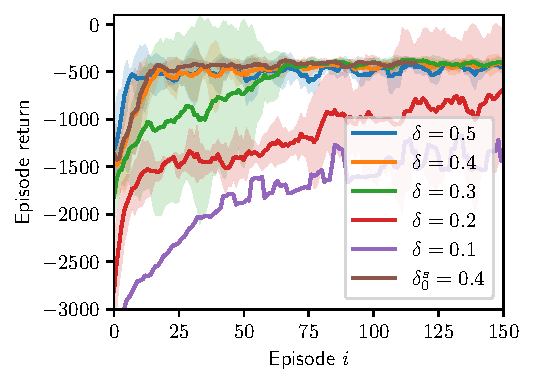
\includegraphics[width=0.95\columnwidth]{../experiments/figures/episode_return_constraint_levels_ablation.pdf}
    \caption{\textbf{Constraint level ablation} Training curves for different constraint levels $\delta$. They show that looser constraints (high $\delta$) have better sample efficiency. They further show that if the constraint is too tight (i.e. $\delta\leq0.2$) then ModeRL gets stuck in local optima and cannot solve the task. Curves show the mean and 95\% confidence interval of the episode return for five random seeds, at each episode $i$ of training. The $\delta^{s}_{0}=4$ experiment used an exponential schedule to tighten the constraint during training. }
    \label{fig-episode_return_constraint_levels_ablation}
\end{figure}

\subsection{Practical Considerations}
\label{sec:org625c4ee}

\textbf{Warm start trajectory optimisation}
In practice, the constrained optimisation in \cref{eq-joint-entropy-objective} fails if the initial trajectory does not satisfy the \(\delta\text{-mode constraint}\).
We overcome this by solving an unconstrained optimisation to a "fake" target state in the initial
state domain \(\stateDomain_{0}\) and using it to warm start our trajectory optimiser.

\textbf{Fixing model parameters during training}
Initially, ModeRL explores the desired dynamic mode and does not observe any state transitions from other modes.
As such, we fix the kernel hyperparameters (e.g. lengthscale and signal variance) associated with the gating network GP.
This prevents the \(\delta\text{-mode-constrained}\) region from expanding significantly further than the observed data.

\textbf{Inducing points}
We initialise each of the sparse GPs with a fixed number of inducing points uniformly sampled from \(\dataset_{0}\).
Although this approach worked well in our experiments, it is unlikely to scale to larger problems.
As such, an interesting direction for future work is to study methods for dynamically adding new inducing points to each GP.

\section{CONCLUSION \label{sec-conclusion}}
\label{sec:orgca252bd}
We introduced ModeRL, a Bayesian model-based RL algorithm for low-dimensional continuous control problems,
that constrains exploration to a single dynamic mode (up to a given probability).
Intuitively, ModeRL relaxes the mode-constrained RL problem in \cref{def-mode-remaining-main}, making it feasible,
whilst still providing "some level" of constraint satisfaction during training.
It uses a nonparametric dynamic model to learn the mode constraint -- as a latent variable -- alongside the dynamic modes.
Importantly, it disentangles the sources of uncertainty in the learned mode constraint.
Our experiments show that our nonparametric formulation of the mode constraint is essential for solving the quadcopter navigation task,
as it enabled our planning algorithm to escape local optima that other strategies could not.

\textbf{Limitations}
The main limitation of ModeRL is that it is restricted to lower dimensional problems,
due to the difficulties of defining GP priors in high dimensions.
Another (potentially unavoidable) downside of ModeRL,
is that it must leave the desired dynamic mode in order to learn about the mode constraint.
This is because we used internal sensing.
However, in some applications, it may be possible to infer the mode constraint using external sensors.
For example, in autonomous driving, it may be possible to infer dynamic modes associated with different road surfaces
without leaving the desired dynamic mode, by using cameras.
Finally, ModeRL uses an open-loop policy.
An interesting direction for future work is to make our algorithm faster so that it can be used to formulate a closed-loop policy via MPC.


\subsubsection*{Acknowledgements}
We thank ST John, Martin Trapp, Arno Solin, and Paul Chang for valuable discussions and feedback.
This work was conducted whilst Aidan Scannell was a PhD student at the EPSRC Centre for Doctoral
Training in Future Autonomous and Robotic Systems (FARSCOPE) at the Bristol Robotics Laboratory.
It was finished whilst funded by the Finnish Center for Artificial Intelligence (FCAI).
\subsubsection*{References}
\printbibliography[heading=none]

\renewcommand{\gatingKernelnM}{\ensuremath{\mode{\hat{k}}(\singleInput, \gatingInducingInput)}}
\renewcommand{\gatingKernelMM}{\ensuremath{\mode{\hat{k}}(\gatingInducingInput, \gatingInducingInput)}}
\renewcommand{\gatingKernelMn}{\ensuremath{\mode{\hat{k}}(\gatingInducingInput, \singleInput)}}
\renewcommand{\gatingKernelnn}{\ensuremath{\mode{\hat{k}}(\singleInput, \singleInput)}}

\renewcommand{\expertKernelnM}{\ensuremath{\mode{k}(\singleInput, \gatingInducingInput)}}
\renewcommand{\expertKernelMM}{\ensuremath{\mode{k}(\gatingInducingInput, \gatingInducingInput)}}
\renewcommand{\expertKernelMn}{\ensuremath{\mode{k}(\gatingInducingInput, \singleInput)}}
\renewcommand{\expertKernelnn}{\ensuremath{\mode{k}(\singleInput, \singleInput)}}

%\clearpage
\appendix

\onecolumn
%\aistatstitle{Mode-Constrained Model-Based Reinforcement Learning via \\Gaussian Processes: Supplementary Materials}
%\thispagestyle{empty}

\section{DYNAMIC MODEL \label{sec-dynamics}}
\label{sec:org5cbcd4b}
This section provides details of our nonparametric dynamic model, including the sparse GP approximations it is
built upon, our GP-based gating network, and how we propagate uncertainty when making multi-step predictions.

\subsection{Sparse Gaussian Processes \label{sec-sparse-approximations}}
\label{sec:orga71e2ee}
Each dynamic mode's predictions conditioned on its inducing variables follows from the properties of multivariate normals
and are given by,
\begin{subequations}  \label{eq-sparse-gp-methodologies}
\begin{align}
&\singleExpertGivenInducing = \E_{\singleLatentExpertGivenInducing} \left[ \singleExpertLikelihood \right] \\
&\singleLatentExpertGivenInducing = \mathcal{N}\left( \mode{\latentFunc}(\singleInput) \mid
\expertKernelnM \expertKernelMM^{-1} \expertInducingOutput,
\expertKernelnn - \expertKernelnM \expertKernelMM^{-1} \expertKernelMn \right),
\end{align}
\end{subequations}
%\normalsize
Similarly for the gating network we have,
\begin{subequations} \label{eq-sparse-gp-methodologies-gating}
\begin{align}
\singleGatingGivenInducing &= \E_{\singleLatentGatingsGivenInducing} \left[ \singleGatingLikelihood \right] \\
\singleLatentGatingsGivenInducing &= \prod_{\modeInd=1}^{\ModeInd} \mathcal{N}\left( \mode{\gatingFunc}(\singleInput) \mid
\gatingKernelnM \gatingKernelMM^{-1} \gatingInducingOutput,
\gatingKernelnn - \gatingKernelnM \gatingKernelMM^{-1} \gatingKernelMn \right),
\end{align}
\end{subequations}

\textbf{Predictive posteriors}
As each GP's inducing variables are normally distributed, the functional form of their predictive posteriors are given by,
\begin{align}
\label{eq--variational-posteriors-functional-experts}
p(\mode{\latentFunc}(\singleInput) \mid \singleInput, \dataset_{0:i})
&\approx \int p(\mode{\latentFunc}(\singleInput) \mid \mode{\latentFunc}(\expertInducingInput))
q(\mode{\latentFunc}(\expertInducingInput)) \text{d} \mode{\latentFunc}(\expertInducingInput)
= \mathcal{N} \left( \mode{\latentFunc}(\singleInput) \mid
\mode{\mathbf{A}} \mode{\mathbf{m}},
\expertKernelnn
+ \mode{\mathbf{A}}
(\mode{\mathbf{S}} - \expertKernelMM)
\mode{\mathbf{A}}^T
\right) \\
p(\GatingFunc(\state_{\timeInd}) \mid \state_{\timeInd}, \dataset_{0:i})
&\approx \prod_{\modeInd=1}^\ModeInd q(\mode{\gatingFunc}(\gatingInducingInput))
= \prod_{\modeInd=1}^\ModeInd \mathcal{N} \left( \mode{\gatingFunc}(\singleInput) \mid
\mode{\hat{\mathbf{A}}} \mode{\hat{\mathbf{m}}},
\gatingKernelnn
+ \mode{\hat{\mathbf{A}}}
(\mode{\hat{\mathbf{S}}} - \gatingKernelMM)
\mode{\hat{\mathbf{A}}}^T
\right), \label{eq--variational-posteriors-functional-gating}
\end{align}

where
\(\mode{\mathbf{A}} = \expertKernelnM \expertKernelMM^{-1}\) and
\(\mode{\hat{\mathbf{A}}} = \gatingKernelnM \gatingKernelMM^{-1}\).
Importantly, our predictive posteriors marginalise the inducing variables in closed form, with Gaussian convolutions.

Given our GP-based gating network, we are able to model the joint distribution over the gating function values \(\desiredGatingFunction(\stateTraj)\)
along a trajectory \(\stateTraj\) with,
\begin{align}
p(\desiredGatingFunction(\stateTraj) \mid \stateTraj, \dataset_{0:i})
&\approx q(\desiredGatingFunction(\stateTraj))
= \mathcal{N} \left(\desiredGatingFunction(\stateTraj) \mid \desiredGatingMeanFunc(\stateTraj),
\desiredGatingCovFunc(\stateTraj, \stateTraj) \right)
\end{align}
where \(\desiredGatingMeanFunc(\cdot)\) and \(\desiredGatingCovFunc(\cdot, \cdot)\) are
sparse GP mean and covariance functions, given by,
%\small
\begin{align}  \label{eq-gating-predictive-eqns}
\desiredGatingMeanFunc(\stateTraj) &=
\desiredGatingKernel(\stateTraj, \gatingInducingInput)
\desiredGatingKernel(\gatingInducingInput, \gatingInducingInput)^{-1}
\hat{\mathbf{m}}_{\desiredMode}  \\
\desiredGatingCovFunc(\stateTraj, \stateTraj) &=
\desiredGatingKernel(\stateTraj, \stateTraj)
+ \desiredGatingKernel(\stateTraj, \gatingInducingInput)
\desiredGatingKernel(\gatingInducingInput, \gatingInducingInput)^{-1}
\left( \hat{\mathbf{S}}_{\desiredMode}
- \desiredGatingKernel(\gatingInducingInput, \gatingInducingInput) \right)
\desiredGatingKernel(\gatingInducingInput, \gatingInducingInput)^{-1}
\desiredGatingKernel(\gatingInducingInput, \stateTraj), \label{eq-joint-gating-covariance}
\end{align}
%\normalsize
where \(\desiredGatingKernel\) and
\(\gatingInducingInput\) are the kernel and inducing inputs
associated with the desired mode's gating function respectively.
This sparse approximation arises because our dynamical model uses sparse GPs and approximates the posterior with,
\begin{align}
q(\desiredGatingFunction(\stateTraj)) = \int p(\desiredGatingFunction(\stateTraj) \mid \desiredGatingFunction(\gatingInducingInput))
q(\desiredGatingFunction(\gatingInducingInput))
\text{d} \desiredGatingFunction(\gatingInducingInput),
\end{align}
where
\(q(\desiredGatingFunction(\gatingInducingInput)) = \mathcal{N}\left( \desiredGatingFunction(\gatingInducingInput \mid \hat{\mathbf{m}}_{\desiredMode}, \hat{\mathbf{S}}_{\desiredMode} \right)\).

\subsection{Gating Network \label{sec-gating-network-app}}
\label{sec:org1505d78}
\textbf{Bernoulli (\(\ModeInd=2\))} Instantiating the model with two dynamic modes, \(\singleModeVar \in \{1, 2\}\), is a special case
where only a single gating function is needed.
This is because the output of a function \(\gatingFunc(\singleInput)\) can be mapped through a sigmoid
function \(\text{sig} : \R \rightarrow [0, 1]\) and interpreted as a probability,
\begin{align} \label{eq-sigmoid}
\Pr(\singleModeVar=1 \mid \gatingFunc(\singleInput)) = \text{sig}(\gatingFunc(\singleInput)).
\end{align}
If this sigmoid function satisfies the point symmetry condition then
the following holds,
\(\Pr(\singleModeVar=2 \mid \gatingFunc(\singleInput)) = 1 - \Pr(\singleModeVar=1 \mid \gatingFunc(\singleInput))\).
This only requires a single gating function and no normalisation term needs to be calculated.
If the sigmoid function in \cref{eq-sigmoid} is selected
to be the Gaussian cumulative distribution function
\(\Phi(\gatingFunc(\cdot)) = \int^{\gatingFunc(\cdot)}_{-\infty} \mathcal{N}(\tau | 0, 1) \text{d} \tau\),
then the mode probability can be calculated in closed form,

\begin{align} \label{eq-mixing-probabilities-analytic}
\Pr(\modeVar_{\timeInd}=1 \mid \singleInput) &=
 \int \Phi\left(\gatingFunc(\singleInput)\right) \mathcal{N}\left(\gatingFunc(\singleInput) \mid \mu_h, \sigma^2_h \right) \text{d} \gatingFunc(\singleInput) \nonumber \\
&= \Phi \left(\frac{\mu_{h}}{\sqrt{1 + \sigma^2_{h} }}\right),
\end{align}
where \(\mu_h\) and \(\sigma^2_{h}\) represent the mean and variance of the gating GP at \(\singleInput\) respectively.

\textbf{Softmax (\(\ModeInd>2\))} In the general case, when there are more than two dynamic modes,
the gating network's likelihood is defined as the Softmax function,
\begin{align} \label{eq-softmax}
\singleGatingLikelihood = \text{softmax}_{\modeInd}\left(\GatingFunc(\singleInput)\right) = \frac{\text{exp}\left(\mode{\gatingFunc}(\singleInput)\right)}{\sum_{j=1}^{\ModeInd} \text{exp}\left(\gatingFunc_j(\singleInput) \right)}.
\end{align}
Each mode's mode probability \(\Pr(\modeVar_{\timeInd}=\modeInd \mid \singleInput)\) is then obtained by marginalising
\textbf{all} of the gating functions.
In the general case where \(\singleGatingLikelihood\) uses the softmax function in
\cref{eq-softmax}, this integral is intractable, so we approximate it with Monte Carlo quadrature.

\begin{figure}
\centering
   \resizebox{0.6\columnwidth}{!}{
    \begin{tikzpicture}[
    pre/.style={<-,shorten <=0.4pt,>=stealth',semithick},
    post/.style={->,shorten >=0.4pt,>=stealth',semithick}
    ]
        \node[const] (x) {$\singleInput$};
        \node[latent, left=of x, yshift=-1.4cm] (f) {$\mode{\latentFunc}(\singleInput)$};
        %\node[latent, right=of x, yshift=-1.7cm] (h) {${h}^{(k)}_n$};
        \node[latent, right=of x, yshift=-1.4cm, xshift=0.5cm] (h) {$\mode{\gatingFunc}(\singleInput)$};

        \node[latent, left=of f, xshift=0.4cm, yshift=0.6cm] (uk) {$\expertInducingOutput$};
        \node[latent, right=of h, xshift=-0.4cm, yshift=0.6cm] (uh) {$\gatingInducingOutput$};
        \node[const, left=of uk, xshift=0.4cm] (zk) {$\expertInducingInput$};
        \node[const, right=of uh, xshift=-0.4cm] (zh) {$\gatingInducingInput$};

        \node[const, left=of f, xshift=0.4cm, yshift=-0.4cm] (thetak) {$\expertParamsK$};
        \node[const, right=of h, xshift=-0.4cm, yshift=-0.4cm] (phik) {$\gatingParamsK$};

        \node[const, below=of thetak, yshift=0.4cm] (sigmak) {$\sigma_{\modeInd}$};

        \node[obs, right=of sigmak, yshift=0.cm, xshift=1.4cm] (y) {$\singleOutput$};
        %\node[latent, right=of y, below=of h] (a) {$\alpha_t$};
        \node[latent, right=of y, xshift=-0.4cm] (a) {$\modeVar_{\timeInd}$};

        %\node[obs, right=of sigmak] (y) {$\Delta\mathbf{x}_{t}$};

        \factor[above=of a] {h-a} {left:Cat} {h} {a};

        \draw[post] (a)--(y);
        \draw[post] (x)-|(f);
        %\draw[post] (f)--(yk);
        \draw[post] (f)--(y);
        %\draw[post] (yk)--(y);
        %\draw[post] (h)--(a);
        \draw[post] (x)-|(h);
        \draw[post] (uk)--(f);
        \draw[post] (uh)--(h);
        \draw[post] (zk)--(uk);
        \draw[post] (zh)--(uh);
        \draw[post] (thetak)--(f);
        \draw[post] (phik)--(h);
        \draw[post] (sigmak)|-(y);

        \plate {} {(x) (y) (a) (f) (h)} {$\TimeInd$};
        %\plate {} {(zk) (uk) (f) (sigmak) (thetak) (yk)} {$K$};
        \plate {} {(zk) (uk) (f) (sigmak) (thetak)} {$\ModeInd$};
        \plate {} {(uh) (h) (phik)} {$\ModeInd$};
    \end{tikzpicture}
    }
\caption{
Graphical model of our augmented dynamic model where each state difference output $\singleOutput$
is generated by mapping the state-action input $\singleInput$ through the latent processes.
The dynamic modes are shown on the left and the gating network on the right.
The generative processes involve evaluating the gating network and sampling a mode indicator variable $\singleModeVar$.
The indicated mode's latent function $\mode{f}$ and noise model $\mathcal{N}(0, \sigma_{\modeInd}^{2})$ are then evaluated to generate the output $\singleOutput$.}
\label{fig-graphical-model-sparse}
\end{figure}

\subsection{Uncertainty Propagation: Moment Matching \label{sec-moment-matching}}
\label{sec:orgad122c5}
To obtain the state distributions \(p(\state_{1} \mid \state_{0}, \action_{0}, \mathcal{D}_{0:i}),\ldots, p(\state_{\TimeInd} \mid \state_{0}, \action_{0:\TimeInd-1}, \mathcal{D}_{0:i})\),
for a given set of actions \(\action_{0},\ldots,\action_{\TimeInd-1}\),
we cascade single-step predictions through the desired dynamic mode's GP using moment matching,
(, a, , a, , a, , a).
That is, we iteratively calculate,
\begin{align}
p(\state_{\timeInd+1} \mid \state_{0}, \action_{0:\timeInd}, \mathcal{D}_{0:i}) = \int \int
\underbrace{p(\state_{\timeInd+1} \mid \dynamicsFunc_{\desiredMode}(\singleInput))}_{\text{Gaussian likelihood}}
\underbrace{p(\dynamicsFunc_{\desiredMode}(\singleInput) \mid \singleInput, \dataset_{0:i})}_{\text{dynamics posterior}}
p(\state_{\timeInd} \mid \state_{0}, \action_{0:\timeInd-1}, \mathcal{D}_{0:i})
\text{d} \dynamicsFunc_{\desiredMode}(\singleInput)
\text{d} \state_{\timeInd},
\end{align}
with \(p(\state_{0}) = \delta(\state_{0})\).
Importantly, the moment-matching approximation allows us to formulate uncertainty propagation using a deterministic
system function,
\begin{align}
\mathbf{z}_{\timeInd+1} = \dynamicsFunc_{\desiredMode}^{\text{MM}}(\mathbf{z}_{\timeInd}, \action_{\timeInd}),
\quad \mathbf{z}_{\timeInd} = [\bm\mu_{\state_{\timeInd}}^{\text{MM}}, \bm\Sigma_{\state_{\timeInd}}^{\text{MM}}],
\end{align}
where \(\bm\mu_{\state_{\timeInd}}^{\text{MM}}\) and \(\bm\Sigma_{\state_{\timeInd}}^{\text{MM}}\) are the mean and covariance of
\(p(\state_{\timeInd} \mid \state_{0}, \action_{0:\timeInd-1}, \mathcal{D}_{0:i})\).
As we use deterministic actions we define the deterministic system function as
\begin{align} \label{eq-moment-matching-system-function}
\mathbf{z}_{\timeInd+1} = \dynamicsFunc_{\desiredMode}^{\text{MM}}(\hat{\mathbf{z}}_{\timeInd}),
\quad \hat{\mathbf{z}}_{\timeInd} = [\bm\mu_{\hat{\state}_{\timeInd}}^{\text{MM}}, \bm\Sigma_{\hat{\state}_{\timeInd}}^{\text{MM}}],
\quad \bm\mu_{\hat{\state}_{\timeInd}}^{\text{MM}} = [\bm\mu_{\state_{\timeInd}}^{\text{MM}}, \action_{\timeInd}],
\quad \bm\Sigma_{\hat{\state}_{\timeInd}}^{\text{MM}} = \text{blkdiag}[\bm\Sigma_{\state_{\timeInd}}^{\text{MM}}, \bm0].
\end{align}

\section{ILLUSTRATIVE EXAMPLE \label{illustrative_example}}
\label{sec:org085e6aa}
\begin{figure}[!t]
    \centering
    %\includegraphics[width=0.5\columnwidth]{./images/quadcopter-problem.png}
    \includegraphics[width=0.5\columnwidth]{./images/quadcopter-problem-blue-red.png}
    \caption{\label{fig-problem-statement} \textbf{Mode-constrained quadcopter navigation} -
    Diagram showing a top-down view of a quadcopter subject to two dynamic modes:
    1) an \textit{operable} dynamic mode (blue) and 2) an \textit{inoperable}, turbulent dynamic mode induced by a strong wind field (red).
    The goal is to navigate to the target state $\targetState$ (white star), whilst avoiding the turbulent dynamic mode (red).}
\end{figure}
ModeRL is tested on a 2D quadcopter navigation example shown in \cref{fig-problem-statement}.
The goal is to fly the quadcopter from an initial state \(\state_0\), to a target state \(\state_{f}\) (white star).
However, it considers a quadcopter operating in an environment subject to spatially varying wind --
induced by a fan -- where two dynamic modes can represent the system,
\begin{description}
\item[{Mode 1}] is an \emph{operable} dynamic mode away from the fan,
\item[{Mode 2}] is an \emph{inoperable}, turbulent dynamic mode in front of the fan.
\end{description}
The turbulent dynamic mode is subject to higher drift (in the negative \(x\) direction) and
to higher diffusion (transition noise).
It is hard to know the exact turbulent dynamics due to complex and uncertain interactions between the
quadcopter and the wind field.
Further to this, controlling the system in the turbulent dynamic mode may be infeasible.
This is because the unpredictability of the turbulence may cause catastrophic failure.
Therefore, when flying the quadcopter to the target state \(\state_{f}\),
it is desirable to find trajectories that avoid entering this turbulent dynamic mode.

The state-space of the velocity-controlled quadcopter example consists of the 2D Cartesian coordinates \(\state = (x, y)\)
and the controls consist of the speed in each direction, given by \(\control = (\velocity_x, \velocity_y)\).

The reward function is given by,
\begin{align} \label{eq-reward-func}
\rewardFunc(\bar{\state}, \bar{\action}) &=
-\left(\state_{\TimeInd} - \targetState \right)^{T}\mathbf{H} \left(\state_{\TimeInd}-\targetState \right)
- \sum_{\timeInd=0}^{\TimeInd-1} \bigg(
\left(\state_{\timeInd} - \targetState \right)^{T}\mathbf{Q} \left(\state_{\timeInd}-\targetState \right)
+\action_{\timeInd}^{T} \mathbf{R} \action_{\timeInd} \bigg)
\\
&=
- \|{\state_{\TimeInd}} - \targetState \|_{\mathbf{H}}
- \sum_{\timeInd=0}^{\TimeInd-1} \bigg( \|{\state_{\timeInd}} - \targetState \|_{\mathbf{Q}}
+ \|\control_{\timeInd} \|_{\mathbf{R}} \bigg)
\end{align}
where \(\mathbf{H}\) and \(\mathbf{Q}\) are user-defined, real symmetric positive semi-definite
weight matrices and \(\mathbf{R}\) is a user-defined, positive definite weight matrix.
In our experiments we set both \(\mathbf{Q}\) and \(\mathbf{R}\) to be the identify matrix \(\mathbf{I}\) and
\(\mathbf{H}\) to be \(100\mathbf{I}\).

\section{EXPERIMENT CONFIGURATION \label{sec-experiment-configuration}}
\label{sec:orgc2b5a12}
This section details how the experiments were configured.

\textbf{Initial data set \(\dataset_0\)}
The initial data set was collected by simulating \(50\) random trajectories with horizon \(\TimeInd=15\) from
the start state \(\state_0 = \{x_{0}, y_{0}\}\) and
terminating them when they left the initial state domain \(\initialStateDomain = \{\state \in \stateDomain \mid x_{0}-1 < x < x_{0}+1, y_{0}-1 < y < y_{0}+1 \}\).

\textbf{Model learning}
In all experiments, the dynamic model was instantiated with \(\ModeInd=2\) modes.
Each dynamic mode's GP used a separate RBF kernel with automatic relevance determination (ARD) for each output dimension \(d\) but
shared its inducing variables for each output dimension \(d\).
Further to this, each dynamic mode learned a separate constant mean function \(c_{\latentFunc_{\modeInd}}\) and separate noise variances for each output dimension.
The gating network used a single gating function with an RBF kernel with ARD and a zero mean function.
An early stopping callback was used to terminate the dynamic model's training.
The early stopping callback used a min delta of \(0\) and a patience of \(50\).
This meant that training terminated after 50 epochs of no improvement.
All of the dynamic model's initial parameters are shown in \cref{tab-params-quadcopter}.
We also fix the kernel hyperparameters (e.g. lengthscale and signal variance) associated with the gating network, along with
the noise variance in the non-desired (turbulent) dynamic mode.


\textbf{Policy}
\todo[inline]{update $\delta$ here and in table}
In all experiments, ModeRL used a horizon of \(\TimeInd=15\) and was configured with \(\delta=0.3\).
At each episode, ModeRL uses the previous solution as the initial solution for the trajectory optimiser.

\textbf{Intrinsic schedule}
In our experiments, we used an exponential decay schedule (with decay rate \(0.96\) and decay steps \(10\)) on the exploration weight \(\beta\).

\begin{table}[htbp]
\caption{\label{tab:orgfb5725e}Experiment configuration and parameter settings.}
\centering
\begin{tabular}{llll}
 & \textbf{DESCRIPTION} & \textbf{SYMBOL} & \textbf{VALUE}\\
\hline
 & Start state & \(\state_{0}\) & \([2.0, -2.5]\)\\
Environment & Target state & \(\targetState\) & \([1.2, 3.0]\)\\
 & Terminal state reward weight & \(\mathbf{H}\) & \(\diag([100, 100])\)\\
 & State reward weight & \(\mathbf{Q}\) & \(\diag([1, 1])\)\\
 & Control reward weight & \(\mathbf{R}\) & \(\diag([1, 1])\)\\
\hline
 & Constraint level & \(\delta\) & \(0.3\)\\
Policy \(\pi\) & Horizon & \(\TimeInd\) & \(15\)\\
 & Exploration weight (initial) & \(\beta_{0}\) & \(10.0\)\\
\hline
 & Batch size & \(\NumData_b\) & \(64\)\\
 & Num epochs & N/A & \(20000\)\\
Dynamics optimiser & Num gating samples & N/A & \(1\)\\
 & Num expert samples & N/A & \(1\)\\
 & Learning rate & N/A & \(0.01\)\\
 & Epsilon & N/A & \(1\times 10^{-8}\)\\
\hline
 & Constant mean function & \(c_{f_{1}}\) & \([0, 0]\)\\
 & Kernel variance (\(d=1\)) & \(\sigma^{2}_{f_{1}}\) & \(1\)\\
 & Kernel lengthscales  (\(d=1\)) & \(l_{f_{1}}\) & \([1, 1, 1, 1]\)\\
Dynamic mode 1 \(f_{1}\) & Kernel variance (\(d=2\)) & \(\sigma^{2}_{f_{1}}\) & \(1\)\\
 & Kernel lengthscales (\(d=2\)) & \(l_{f_{1}}\) & \([1, 1, 1, 1]\)\\
 & Likelihood variance & \(\sigma^{2}_{1}\) & \(\diag([1, 1])\)\\
 & Num inducing points & \(\NumInducing_{f_{1}}\) & \(50\)\\
 & Inducing inputs & \(\expertsInducingInput_1\) & \(\expertsInducingInput_1 \subseteq \allInput_{0}\) with \(\#\expertsInducingInput_1 = \NumInducing\)\\
\hline
 & Constant mean function & \(c_{f_{2}}\) & \([0,0]\)\\
 & Kernel variance (\(d=1\)) & \(\sigma^{2}_{f_{2}}\) & \(1\)\\
 & Kernel lengthscales  (\(d=1\)) & \(l_{f_{2}}\) & \([1, 1, 1,1]\)\\
Dynamic mode 2 \(f_{2}\) & Kernel variance (\(d=2\)) & \(\sigma^{2}_{f_{2}}\) & \(1\)\\
 & Kernel lengthscales (\(d=2\)) & \(l_{f_{2}}\) & \([1, 1, 1,1]\)\\
 & Likelihood variance & \(\sigma^{2}_{2}\) & \(\diag([1,1])\)\\
 & Num inducing points & \(\NumInducing_{f_{2}}\) & \(50\)\\
 & Inducing inputs & \(\expertsInducingInput_2\) & \(\expertsInducingInput_2 \subseteq \allInput_{0}\) with \(\#\expertsInducingInput_2 = \NumInducing\)\\
\hline
 & Kernel variance & \(\sigma^{2}_{h_{1}}\) & \(1\)\\
 & Kernel lengthscales & \(l_{h_{1}}\) & \([0.8, 0.8]\)\\
Gating function 1 \(h_{1}\) & Active dims & N/A & \([0, 1]\)\\
 & Num inducing points & \(\NumInducing_{h_{1}}\) & \(90\)\\
 & Inducing inputs & \(\gatingInducingInput\) & \(\gatingInducingInput \subseteq \allInput_{0}\) with \(\#\gatingInducingInput = \NumInducing_{h}\)\\
\end{tabular}
\end{table}

\newpage

\section{FURTHER EXPERIMENTS}
\label{sec:orgfa9747a}
\begin{figure}[h]
    \centering
    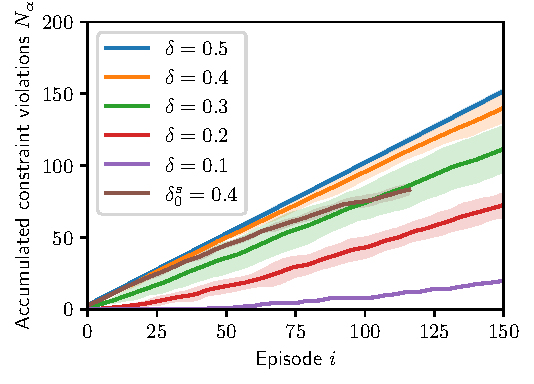
\includegraphics[width=0.5\textwidth]{../experiments/figures/num_constrint_violations_constraint_levels_ablation.pdf}
    %\caption{\textbf{Constraint level ablation} Shows how the constraint level $\delta$ influences the number of constraint violations during training. Specifically, it shows the accumulated number of constraint violations ($N^{\modeVar}_{i}$) at each episode ($i$) during training, for five constraint levels $\delta$.
    %Results show mean and 95\% confidence interval for five random seeds.}
    \caption{\textbf{Constraint level ablation} Accumulated number of constraint violations at each episode $i$ of training, for different constraint levels $\delta$.
    It shows that tighter constraints (i.e. lower $\delta$) result in less constraint violations during training.
    Lines show the mean and 95\% confidence interval of the accumulated number of constraint violations for five random seeds, at each episode $i$ of training. The $\delta^{s}_{0}=4$ experiment used an exponential schedule to tighten the constraint during training. }
    \label{fig-num_constrint_violations_constraint_levels_ablation}
\end{figure}
\end{document}